%=====================================================================
%  Two Scales of Decision: Federated Intent-Driven QoS Orchestration
%  Across Autonomous Cloud--Edge Providers
%
%  Compile:  pdflatex paper && bibtex paper && pdflatex paper x2
%=====================================================================
\documentclass[conference]{IEEEtran}
\IEEEoverridecommandlockouts

\usepackage{cite}
\usepackage{amsmath,amssymb,amsfonts}
\usepackage{algorithmic}
\usepackage{graphicx}
\usepackage{textcomp}
\usepackage{xcolor}
\usepackage{booktabs}
\usepackage{url}
\usepackage{tabularx}
\usepackage{multirow}
\usepackage{stfloats}   % allows full-width floats at the bottom of a page
\usepackage{tikz}
\usetikzlibrary{positioning,shapes.geometric,fit,arrows.meta,calc,backgrounds}

% --- Drafting aids: remove before submission -------------------------
\newcommand{\todo}[1]{\textcolor{red}{\textbf{[TO COMPLETE: #1]}}}
\newcommand{\refcheck}[1]{\textcolor{blue}{\textbf{[REF TO VERIFY: #1]}}}
% ---------------------------------------------------------------------

\def\BibTeX{{\rm B\kern-.05em{\sc i\kern-.025em b}\kern-.08em
    T\kern-.1667em\lower.7ex\hbox{E}\kern-.125emX}}

\begin{document}

\title{Two Scales of Decision: Federated Intent-Driven QoS\\
       Orchestration Across Autonomous Cloud--Edge Providers}

\author{
\IEEEauthorblockN{Ahmed Kammoun\IEEEauthorrefmark{1},
                  Sami Yangui\IEEEauthorrefmark{2},
                  Samir Medjiah\IEEEauthorrefmark{2},
                  Imene Lahyani\IEEEauthorrefmark{1},
                  Mustapha Amine Kechaou\IEEEauthorrefmark{1}}
\IEEEauthorblockA{\IEEEauthorrefmark{1}\todo{affiliation~1 --- ENIS,
                  University of Sfax, Tunisia?}\\
                  \todo{emails}}
\IEEEauthorblockA{\IEEEauthorrefmark{2}\todo{affiliation~2 --- LAAS-CNRS,
                  Universit\'e de Toulouse, CNRS, INSA, Toulouse, France?}\\
                  \todo{emails}}
}

\maketitle

\begin{abstract}
Applications in the cloud--edge continuum increasingly span several
administrative domains, yet placement decisions stop at the boundary of a
single provider. We identify a structural reason: multi-criteria ranking
methods such as TOPSIS normalise over the pool of candidates they are given,
so a closeness score means ``best here'' and carries no information about
absolute quality. Two providers ranking their own machines therefore produce
numbers that cannot be compared. We present \textsc{xQoS}, a federated
intent-driven QoS orchestrator that separates the two decisions: TOPSIS ranks
candidates \emph{within} a provider, while an augmented Tchebycheff
scalarisation over the primary objectives---measured against the thresholds
providers share---compares \emph{across} them. Providers negotiate through a
master-less Contract Net whose currency is a QoS shortfall rather than a
price. A large language model translates a natural-language objective into a
weighted SLO contract by inferring the class of service it implies, and
mutual information promotes correlated metrics to secondary objectives. On a
hardware-in-the-loop testbed of four OpenStack virtual machines exposing
eight placement targets, driven by a mobile consumer, enabling the federation
reduces the share of the lap spent in SLO violation from $54.8\%$ to
$23.8\%$ over four runs per condition ($p=0.029$, exact Mann--Whitney);
against an oracle at $7.5\%$ and a static placement at $81.9\%$, the system
captures roughly $78\%$ of the achievable improvement. Twelve intents drawn
from a third-party document exercise the translation, including two the
system correctly declines. We also report where the approach falls short, including translated
thresholds that reflect the language model's prior rather than the
deployment; a mutual-information signal absent on the original testbed by
construction is subsequently confirmed once load and latency are causally
coupled.
\end{abstract}

\begin{IEEEkeywords}
cloud--edge continuum, intent-based orchestration, quality of service,
multi-criteria decision making, federated orchestration, large language
models, service placement
\end{IEEEkeywords}

%=====================================================================
\section{Introduction}
\label{sec:intro}

Modern cyber-physical applications---autonomous vehicles, Industry~5.0
production lines, real-time infrastructure monitoring---no longer execute
inside a single administrative domain. They run across a \emph{cloud
continuum} in which cloud operators, edge and fog providers, IoT verticals
and private infrastructures each contribute a fraction of the resources.
End-to-end quality of service (QoS) therefore depends on the coordination of
actors that share no scheduler, no monitoring plane, and no common notion of
what a ``good'' placement is~\cite{mouradian2018,belcastro2025}.

Production orchestrators do not address this setting. Kubernetes and its
scheduling extensions assume one cluster under one authority: placement is
decided once, from resource requests, and the scheduler is blind to the
network latency towards a moving consumer. SLO-aware orchestration
systems~\cite{metsch2023,qonnect2025} relax this by reacting to measured
violations, but they remain single-domain. Intent-based
management~\cite{morichetta2023,sfaxi2026policies} raises the
abstraction level of the operator's request, yet stops at the boundary of a
single provider.

Closing this gap raises three problems, which this paper addresses in order.

\textbf{Expressing the objective.} An operator does not want to specify a
placement; they want to state a goal---\emph{``alert me immediately if the
site goes down''}. Turning such a sentence into numeric, weighted, comparable
QoS constraints is a translation problem, not a configuration one. Keyword
matching fails on sentences that contain no metric, no number and no
technical term.

\textbf{Deciding before the breach.} An orchestrator that migrates
\emph{after} an SLO is violated is structurally late: by the time the
violation is measured, the user has already experienced it. Deciding on a
\emph{prediction} rather than on a measurement is what makes orchestration
proactive.

\textbf{Comparing what is not comparable.} This is the problem we consider
central. Multi-criteria decision methods such as TOPSIS~\cite{hwang1981}
normalise each criterion over the pool of candidates they are given, and the
MCDM community has long studied the consequence under the name \emph{rank
reversal}~\cite{belton1983,garciacascales2012}. We take that known property
one step further, into a setting where it stops being a robustness concern
and becomes a correctness one: a closeness score of $0.87$ means
\emph{``best among these''}, and the best candidate of \emph{any} pool scores
close to $1.0$ regardless of its absolute quality. Two providers ranking
their own machines therefore produce numbers that are not on a common scale
at all. Selecting a host across providers requires a quantity measured
against \emph{absolute} thresholds, together with a protocol that no single
actor controls---failing which multi-provider orchestration silently
degrades into a hierarchy with a master.

We present \textsc{xQoS}, a federated intent-driven QoS orchestrator in which
every provider runs a complete and autonomous orchestration stack. A business
objective expressed in natural language is translated into a weighted SLO
contract, enriched with statistically discovered secondary objectives,
evaluated against machine-learning predictions for every candidate host, and
resolved locally by TOPSIS. When no local host satisfies the contract,
providers negotiate through a Contract Net protocol whose currency is a
threshold-relative \emph{Gap Grade}---the only quantity that remains
meaningful across pools.

The contributions of this paper are the following.

\begin{enumerate}
    \item \textbf{A two-scale placement decision.} We show why a
    pool-relative multi-criteria score cannot cross a provider boundary, and
    separate the two decisions accordingly: TOPSIS ranks candidates
    \emph{within} a provider, while an augmented Tchebycheff
    scalarisation~\cite{steuer1983} over the primary SLOs,
    evaluated against absolute thresholds, compares \emph{across} providers.
    The two scores carry opposite polarities and are never mixed.

    \item \textbf{A master-less arbitration protocol.} Any provider that
    detects a violation becomes the initiator of a Contract Net
    round~\cite{smith1980}: it broadcasts a call for proposals, bids on
    its own resources, and applies the arbiter's verdict. Initiator is a
    role, not a fixed coordinator. An absolute dead-band prevents an
    incumbent provider from being displaced by a marginal improvement.

    \item \textbf{Intent-to-contract translation by service-type inference.}
    A large language model is prompted to identify the class of service that
    would fulfil the stated intention and to derive its QoS needs, rather
    than to extract values from the sentence. The same inference assigns each
    objective a weight and selects how the resulting contract is merged with
    the active one. A schema validation stage bounds the non-determinism of
    the model.

    \item \textbf{Self-supervised contract enrichment, and a negative result
    on it.} Continuous mutual information, estimated with a
    $k$-nearest-neighbour estimator~\cite{kraskov2004}, is computed between
    each observed metric and the binary violation signal; metrics whose
    relative score exceeds a threshold are promoted to weighted secondary
    objectives, giving the system constraints no operator declared. We also
    report that on our testbed these scores do not survive a null hypothesis
    preserving the autocorrelation of the series: the workload generator
    makes resource usage independent of the latency that drives violations,
    so there is no dependency to discover. A positive control on synthetic
    series confirms the estimator and null test detect a real dependency
    when one is constructed, so the absence of signal reflects the workload
    generator rather than a limitation of the method---we state this
    rather than claim a result the testbed does not support.

    \item \textbf{An implementation and its experimental evaluation.} The
    prototype comprises about $12\,300$ lines of Python across twelve
    microservices per provider, with a further $6\,100$ lines of tests, and is
    evaluated on a hardware-in-the-loop testbed: four OpenStack virtual
    machines under Kubernetes expose eight independently addressable placement
    targets, and every elected placement is applied as a real pod migration
    through the Kubernetes API. QoS is emulated at the target---latency is
    derived from the distance to a mobile consumer whose trajectory is driven
    by a PiCar-X simulator, CPU and memory follow a bounded random walk. The
    testbed geometry is dimensioned so that no single provider can serve the
    consumer for a full lap, making inter-provider handover a structural
    necessity rather than a staged event.
\end{enumerate}

The remainder of this paper is organised as follows.
Section~\ref{sec:related} positions our work with respect to the state of the
art. Section~\ref{sec:overview} presents the system architecture and
Section~\ref{sec:design} its orchestration cycle.
Section~\ref{sec:method} details the four decision mechanisms.
Section~\ref{sec:eval} reports the experimental evaluation.
Section~\ref{sec:discussion} discusses the limitations of the approach, and
Section~\ref{sec:conclusion} concludes.

%=====================================================================
% NOTE: Fig. 1 is declared here, ahead of the section that discusses it
% (Sec. III), so that LaTeX can place it at the top of an early page.
% Full-width floats can only be set at the top of a page that follows their
% declaration point.
\begin{figure*}[!t]
\centering
\resizebox{0.94\textwidth}{!}{% Figure 1 --- xQoS architecture: two symmetric providers over a
% transversally partitioned infrastructure.
% Included from paper.tex. Requires: tikz + positioning, shapes.geometric,
% fit, arrows.meta, calc, backgrounds.

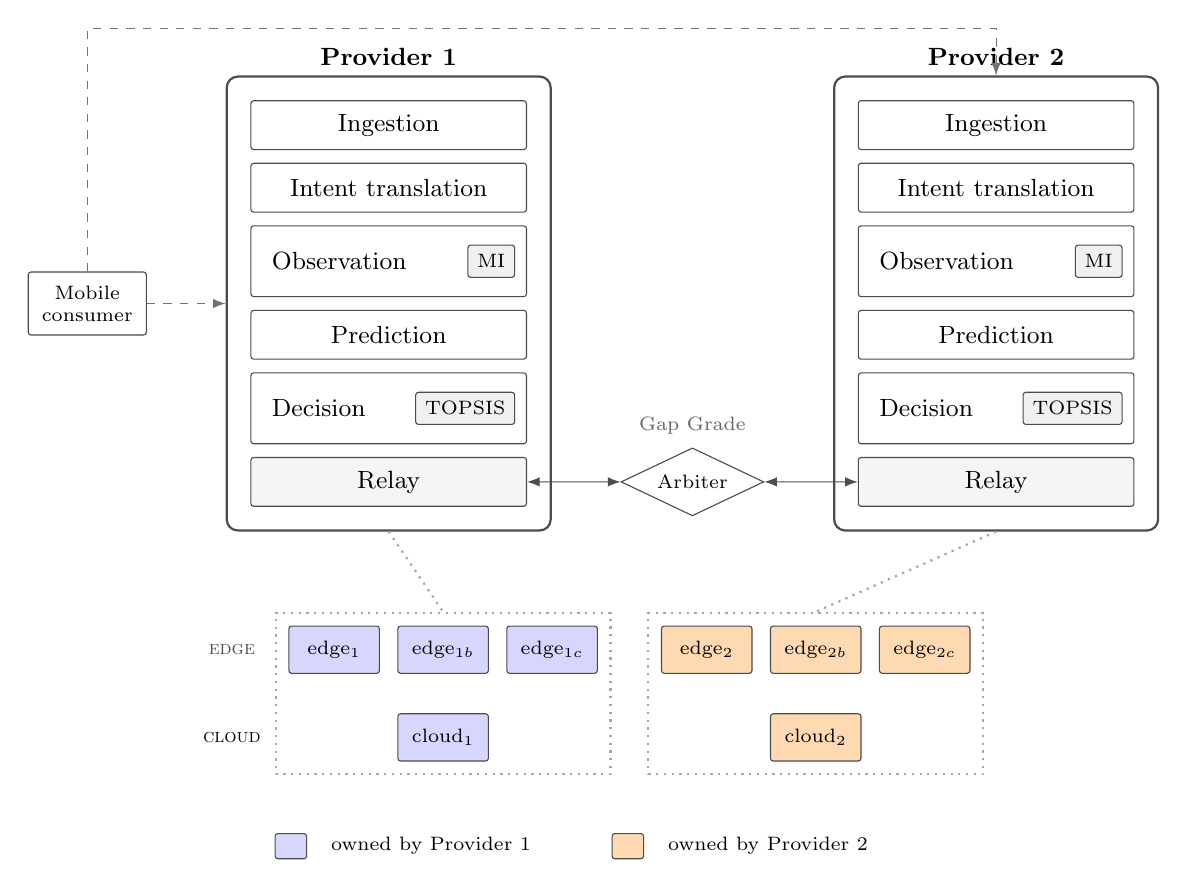
\begin{tikzpicture}[
    font=\small,
    blk/.style   = {draw=black!70, rounded corners=1pt, minimum width=3.5cm,
                    minimum height=6.2mm, align=center, fill=white},
    prov/.style  = {draw=black!70, rounded corners=4pt, thick, inner sep=3mm},
    node distance = 1.6mm,
    vm/.style    = {draw=black!70, minimum width=1.15cm, minimum height=6mm,
                    rounded corners=1pt, align=center, font=\scriptsize},
    p1/.style    = {vm, fill=blue!16},
    p2/.style    = {vm, fill=orange!30},
    lnk/.style   = {-{Latex[length=1.6mm]}, draw=black!60},
    dlnk/.style  = {-{Latex[length=1.6mm]}, dashed, draw=black!55},
    own/.style   = {draw=black!35, dotted, thick},
]

%============================ PROVIDER 1 ============================
\node[blk] (a1) {Ingestion};
\node[blk, below=of a1] (a2) {Intent translation};
\node[blk, below=of a2, minimum height=9mm] (a3) {};
\node[anchor=west] at ([xshift=1.5mm]a3.west) {Observation};
\node[draw=black!70, fill=black!6, rounded corners=1pt, font=\scriptsize,
      inner sep=1.2mm, anchor=east] (mi1) at ([xshift=-1.5mm]a3.east) {MI};
\node[blk, below=of a3] (a4) {Prediction};
\node[blk, below=of a4, minimum height=9mm] (a5) {};
\node[anchor=west] at ([xshift=1.5mm]a5.west) {Decision};
\node[draw=black!70, fill=black!6, rounded corners=1pt, font=\scriptsize,
      inner sep=1.2mm, anchor=east] (t1) at ([xshift=-1.5mm]a5.east) {TOPSIS};
\node[blk, below=of a5, fill=black!4] (r1) {Relay};

\node[prov, fit=(a1)(r1), label={[font=\small\bfseries]above:Provider 1}]
      (P1) {};

%============================ PROVIDER 2 ============================
\node[blk, right=4.2cm of a1] (b1) {Ingestion};
\node[blk, below=of b1] (b2) {Intent translation};
\node[blk, below=of b2, minimum height=9mm] (b3) {};
\node[anchor=west] at ([xshift=1.5mm]b3.west) {Observation};
\node[draw=black!70, fill=black!6, rounded corners=1pt, font=\scriptsize,
      inner sep=1.2mm, anchor=east] (mi2) at ([xshift=-1.5mm]b3.east) {MI};
\node[blk, below=of b3] (b4) {Prediction};
\node[blk, below=of b4, minimum height=9mm] (b5) {};
\node[anchor=west] at ([xshift=1.5mm]b5.west) {Decision};
\node[draw=black!70, fill=black!6, rounded corners=1pt, font=\scriptsize,
      inner sep=1.2mm, anchor=east] (t2) at ([xshift=-1.5mm]b5.east) {TOPSIS};
\node[blk, below=of b5, fill=black!4] (r2) {Relay};

\node[prov, fit=(b1)(r2), label={[font=\small\bfseries]above:Provider 2}]
      (P2) {};

%============================ ARBITER ===============================
\coordinate (mid) at ($(r1.east)!0.5!(r2.west)$);
\node[draw=black!70, diamond, aspect=2.1, inner sep=0.9mm, fill=white,
      font=\scriptsize] (arb) at (mid) {Arbiter};
\draw[{Latex[length=1.6mm]}-{Latex[length=1.6mm]}, draw=black!70]
      (r1.east) -- (arb.west);
\draw[{Latex[length=1.6mm]}-{Latex[length=1.6mm]}, draw=black!70]
      (arb.east) -- (r2.west);
\node[font=\scriptsize, above=0.4mm of arb, text=black!60]
      {Gap Grade};

%============================ VEHICLE ===============================
\node[draw=black!70, rounded corners=1pt, minimum width=1.5cm,
      minimum height=8mm, align=center, font=\scriptsize,
      left=1.0cm of P1.west] (car) {Mobile\\consumer};
\draw[dlnk] (car.east) -- ++(0.45,0) |- (P1.west);
\draw[dlnk] (car.north) |- ([yshift=6mm]$(P1.north)!0.5!(P2.north)$) -| (P2.north);

%======================= INFRASTRUCTURE LAYER =======================
\coordinate (base) at ([yshift=-1.5cm]$(P1.south)!0.5!(P2.south)$);

% --- edge row: 3 VMs per provider
\node[p1] (e1)  at ([xshift=-4.55cm]base) {edge$_1$};
\node[p1, right=2.2mm of e1]  (e1b) {edge$_{1b}$};
\node[p1, right=2.2mm of e1b] (e1c) {edge$_{1c}$};
\node[p2, right=8mm of e1c]   (e2)  {edge$_2$};
\node[p2, right=2.2mm of e2]  (e2b) {edge$_{2b}$};
\node[p2, right=2.2mm of e2b] (e2c) {edge$_{2c}$};

% --- cloud row: 1 VM per provider, aligned under its own group
\node[p1, below=5mm of e1b] (c1) {cloud$_1$};
\node[p2, below=5mm of e2b] (c2) {cloud$_2$};

\node[font=\scriptsize, left=3mm of e1, text=black!70] (lblE) {\textsc{edge}};
\node[font=\scriptsize] at (lblE |- c1) {\textsc{cloud}};

% --- ownership envelopes (this is what makes the partition readable)
\node[own, fit=(e1)(e1c)(c1), inner sep=1.6mm] (own1) {};
\node[own, fit=(e2)(e2c)(c2), inner sep=1.6mm] (own2) {};

\draw[own] (P1.south) -- (own1.north);
\draw[own] (P2.south) -- (own2.north);

%============================ LEGEND ================================
\node[p1, minimum width=4mm, minimum height=3.2mm, anchor=west]
      (lg1) at ([yshift=-9mm]own1.south west) {};
\node[font=\scriptsize, anchor=west] (lg1t)
      at ([xshift=1.8mm]lg1.east) {owned by Provider 1};
\node[p2, minimum width=4mm, minimum height=3.2mm, anchor=west]
      (lg2) at ([xshift=9mm]lg1t.east) {};
\node[font=\scriptsize, anchor=west]
      at ([xshift=1.8mm]lg2.east) {owned by Provider 2};

\end{tikzpicture}
}
\caption{\textsc{xQoS} architecture. Two providers run identical and
independent orchestration stacks; the symmetry is the point, as no provider
holds a coordinating role. Mutual information (MI) widens the contract inside
Observation; TOPSIS then ranks candidates on that full contract, strictly
inside a provider, on that provider's own candidates; the Gap Grade is the
only quantity that crosses the relay link. The infrastructure partition is
\emph{transversal}: each provider owns machines in both the edge and the
cloud tier, so a provider cannot be summarised as ``the near one''.}
\label{fig:architecture}
\end{figure*}

\section{Related Work}
\label{sec:related}

We review five lines of work that each address part of the problem, and
identify what none of them provides.

\subsection{QoS-aware placement in the continuum}

Service placement under QoS constraints is a mature problem. Skarlat
\emph{et al.}~\cite{skarlat2017} formulate fog service placement as an
optimisation model and report a 35\% cost reduction over a cloud-only
deployment. More recent systems make the decision \emph{proactive}: Sfaxi
\emph{et al.}~\cite{sfaxi2024tnsm} forecast latency degradation with
exponential smoothing, compare it to ARIMA, and re-place the decision module
of an autonomous car before the threshold is crossed; the same group extends
the approach to interdependent services under shared resource
constraints~\cite{sfaxi2025aidriven}. Others operate directly on Kubernetes:
Rosmaninho \emph{et al.}~\cite{rosmaninho2024} add a location-aware resource
definition and a custom scheduler for a smart-city testbed, and
QONNECT~\cite{qonnect2025} extends QoS-aware orchestration to distributed
Kubernetes clusters. Di Cicco \emph{et al.}~\cite{dicicco2025} approximate the
Pareto front of orchestration policies with multi-objective reinforcement
learning, letting an operator choose a trade-off \emph{a posteriori}.

All of these decide over a single pool of candidates, under a single
authority. The question of what happens when the pool is split across
mutually autonomous owners is not raised.

\subsection{Intent-based management}

Intent-based systems raise the abstraction level of the operator's request.
Metsch \emph{et al.}~\cite{metsch2023} add an SLO planning component to a
Kubernetes stack, so that service owners declare target KPIs instead of
resource requests. Morichetta \emph{et al.}~\cite{morichetta2023} deploy an
intent-based system over the serverless continuum and show that it can
resolve conflicting objectives such as efficiency versus availability.
Akbari \emph{et al.} use LLMs both to emulate intent-based
scheduling~\cite{akbari2024icontinuum} and to perform root-cause analysis
when an intent is violated~\cite{akbari2025intentcontinuum}. The same
abstraction has been applied to end-to-end networking~\cite{velasco2023} and,
recently, to network isolation policies~\cite{pizzato2026}.

Closest to our work, Sfaxi \emph{et al.}~\cite{sfaxi2026policies} propose an
LLM-driven multi-agent architecture---intent mining, telemetry, forecasting,
an LLM-augmented reasoner and a QoS management agent---that translates
user-expressed intents into proactive placement decisions, and ground it with
a MILP formulation of the same problem. We build directly on this line of
work. The architecture we present shares its premise, that QoS management
should start from the user's intent rather than from system-centric policies,
and extends it along the axis it does not address: all of these systems,
including~\cite{sfaxi2026policies}, operate within a single administrative
domain.

\subsection{Multi-criteria decision making for placement}

Placement is inherently multi-criteria, and multi-criteria decision making
(MCDM) methods are an established tool for it. TOPSIS~\cite{hwang1981} in
particular has been applied to edge resource allocation~\cite{topsis2022edge},
ranking candidates by their relative closeness to an ideal solution. We use
TOPSIS as well, and claim no novelty in doing so.

That the resulting score depends on the set of alternatives is not a new
observation. The MCDM community has studied it for decades under the name
\emph{rank reversal}: adding or removing an alternative can change the
relative order of the others, because the normalisation step is computed over
the candidate set itself. Belton and Gear~\cite{belton1983} identified the
phenomenon in the analytic hierarchy process, and it has since been
characterised specifically for TOPSIS~\cite{garciacascales2012}. We claim no
discovery here.

What we do claim is a consequence that the placement literature does not draw.
Rank reversal is usually treated as a robustness concern---a ranking that
ought to be stable is not. In a federated setting the implication is
stronger and different in kind: because each provider normalises over its own
pool, the top candidate of \emph{any} pool scores close to $1$ whatever its
absolute quality, so two providers' scores are not merely unstable with
respect to one another, they are \emph{not defined on a common scale at all}.
Comparing them is not an approximation to be bounded but an operation without
meaning. As long as one authority decides over one pool this is harmless; it
becomes a correctness problem the moment placement crosses a provider
boundary, and to the best of our knowledge no placement work states it in
those terms.

\subsection{Multi-domain and federated orchestration}

Orchestration across administrative domains has been identified as an open
challenge for a decade~\cite{nextgen2018}. Practical answers have largely been
market-shaped: NECOS and 5GEx introduce a marketplace where domains
advertise, negotiate and sell resources for network slices~\cite{nextgen2018},
service function chains are customised across
domains~\cite{sfcmultidomain2023}, and a recent federated-market
substrate~\cite{federatedmarket2026} lets autonomic brokers converge through
marginal-cost price signals.

Two properties separate these approaches from ours. First, a marketplace or
broker is a coordination point, and therefore a \emph{de facto} master; we
require that any provider be able to initiate a round. Second, and more
fundamentally, their currency is economic. A price presupposes inter-provider
accounting, which a QoS federation does not necessarily have. Our currency is
a QoS shortfall measured against the SLO thresholds the providers already
share.

\subsection{Foundations}

Our work rests on four classical results: the autonomic computing
vision~\cite{kephart2003}, whose MAPE-K loop the orchestration cycle
instantiates; the Contract Net protocol~\cite{smith1980}, from which we take
initiator as a role rather than a fixed coordinator; the augmented
Tchebycheff scalarisation~\cite{steuer1983}, whose pessimistic $\max$ term is
what prevents a provider from hiding one bad metric behind several good ones;
and the $k$-nearest-neighbour mutual information
estimator~\cite{kraskov2004}, which lets us measure dependence between
continuous metrics and a binary violation signal without discretisation.
Broader context on the continuum is given by the surveys of Mouradian
\emph{et al.}~\cite{mouradian2018} and Belcastro
\emph{et al.}~\cite{belcastro2025}.

\subsection{Positioning}

Table~\ref{tab:related} summarises the comparison. Existing work translates
intents, predicts degradation, and ranks candidates---but always over one
pool, under one authority. No approach we are aware of addresses the case in
which two autonomous orchestrators must compare placements that their
respective ranking methods make structurally incomparable.

\begin{table*}[!t]
\centering
\caption{Positioning of \textsc{xQoS} with respect to the closest work.}
\label{tab:related}
\footnotesize
\renewcommand{\arraystretch}{1.2}
\setlength{\tabcolsep}{4pt}
\begin{tabularx}{\textwidth}{@{}p{3.05cm} X X X p{1.75cm} X@{}}
\toprule
\textbf{Work} & \textbf{Intent input} & \textbf{Anticipation} &
\textbf{Decision method} & \textbf{Multi-prov.} & \textbf{Validation}\\
\midrule
Metsch \emph{et al.}~\cite{metsch2023}
  & declared SLOs & --- & planner over K8s & no & K8s testbed \\
Morichetta \emph{et al.}~\cite{morichetta2023}
  & intent, 3-layer model & --- & rule-based conflict resolution & no
  & AWS PoC + simulation \\
Akbari \emph{et al.}~\cite{akbari2025intentcontinuum}
  & natural language (LLM) & root-cause analysis & LLM reasoning & no
  & SDN emulation \\
Sfaxi \emph{et al.}~\cite{sfaxi2024tnsm}
  & --- & exp.\ smoothing / ARIMA & threshold on forecast & no
  & simulation \\
Sfaxi \emph{et al.}~\cite{sfaxi2026policies}
  & voice, natural language & forecasting agent & LLM reasoner + MILP & no
  & datasets + expert study \\
Federated market~\cite{federatedmarket2026}
  & --- & --- & marginal-cost price signals & yes, brokers & simulation \\
\addlinespace[2pt]
\textbf{\textsc{xQoS} (this work)}
  & natural language (LLM) & ML prediction + MI-discovered SLOs
  & TOPSIS (local) + Gap Grade (global) & \textbf{yes, master-less}
  & \textbf{physical testbed} \\
\bottomrule
\end{tabularx}
\end{table*}

\section{System Overview}
\label{sec:overview}

\subsection{Design principles}

Four principles shape the architecture shown in
Fig.~\ref{fig:architecture}.

\emph{Complete autonomy.} Each provider runs an entire orchestration stack.
No component on the decision path is shared: a provider builds its own SLO
contract, collects its own metrics, produces its own predictions and ranks
its own candidates. A provider cut off from the federation keeps orchestrating
its own resources; it degrades, it does not stop. The one element both
providers read is the infrastructure control plane, which reports where the
service actually runs---a source of truth, not a decision maker.
Section~\ref{sec:discussion} returns to this dependency.

\emph{State isolation.} Each provider owns its metric histories, its active
contract and its decision log. No data structure is shared between providers;
the relay is the only inter-provider channel.

\emph{Registry-driven configuration.} QoS metrics are declared once, in a
single registry that every stage iterates over---collection, mutual
information, prediction, ranking. Adding a QoS dimension is a declaration, not
a refactoring.

\emph{Graceful degradation.} The failure of one element narrows the decision
rather than blocking it: without predictions the system falls back to measured
values, without a reachable peer the federation reduces to a single provider,
and an unsatisfiable contract yields an explicit infeasible outcome rather
than an arbitrary placement.

\subsection{Anatomy of a provider}

A provider is organised as a hub-and-spoke: a core sequences the cycle and
every functional block answers to it, so no two blocks communicate directly.
This is what makes a cycle traceable end to end, and what allows each stage to
be profiled independently. Five blocks are relevant to the reader:

\begin{itemize}
    \item \textbf{Ingestion} receives QoS measurements from the consumer and
    triggers a cycle.
    \item \textbf{Intent translation} turns a natural-language objective into
    a weighted SLO contract (Section~\ref{sec:intent}).
    \item \textbf{Observation} collects per-machine metrics, maintains their
    histories, and derives secondary objectives by mutual information
    (Section~\ref{sec:mi}).
    \item \textbf{Prediction} produces the future value of each metric for
    every candidate machine.
    \item \textbf{Decision} detects violations, ranks the compliant local
    candidates with TOPSIS over the full contract---primary objectives and
    any secondary ones Observation derived---and, when no local candidate
    qualifies, enters inter-provider arbitration.
\end{itemize}

\subsection{The transversal partition}

Provider identity and infrastructure tier are orthogonal. As
Fig.~\ref{fig:architecture} shows, each provider owns machines at the edge
\emph{and} in the cloud. This is a deliberate design decision, and the paper
depends on it.

Had one provider been the edge and the other the cloud, inter-provider
selection would collapse into a tier choice: take the edge when latency
matters, the cloud otherwise. No arbitration would be needed, because the
answer would be readable from the topology. The transversal partition removes
that shortcut. Both providers can serve the consumer, both can fail to, and
which one is preferable at a given instant is a genuine question about
absolute QoS---which is precisely what the Gap Grade answers.

\subsection{Federation state}

At any instant, the provider whose machine hosts the service is
\textsc{active}; the other is \textsc{standby}.

The role is \emph{not} negotiated. Each provider asks the infrastructure
control plane which machine currently hosts the service, and compares that
machine's owner with its own identity. Being \textsc{active} is therefore an
observation, not an assignment, and the federation needs no distributed
consensus to agree on it: a single service instance runs in a single place,
so two providers cannot both believe they are \textsc{active}. The only
subtlety is the propagation delay after a migration, during which a newly
promoted provider ignores infrastructure readings that still name the previous
host; without this guard the role would oscillate for the duration of the
migration.

Two rules complete the federation state. First, all inter-orchestrator traffic
passes through the relays: a provider's decision core is never addressable by
a peer, which keeps the interaction surface to a documented set of messages.
Second, a \textsc{standby} that receives a broadcast \emph{adopts} the
initiator's contract in full---primary and secondary objectives, with their
weights---instead of recomputing one of its own. This is not a convenience.
Two providers evaluating against two different contracts would produce two Gap
Grades measured against different thresholds, and comparing them would be
meaningless. Contract adoption is what makes the comparison in
Section~\ref{sec:gap} legitimate.

\subsection{The orchestration cycle}

A cycle is triggered by the arrival of a measurement batch, never by a timer,
and cycles never overlap: a batch arriving while a cycle is in flight is
dropped rather than queued, so the system always decides on the freshest
observation rather than on a backlog. Section~\ref{sec:design} details the
stages.

\section{Orchestration Cycle}
\label{sec:design}

\begin{figure}[!t]
\centering
\resizebox{0.86\columnwidth}{!}{% Figure 2 --- the orchestration cycle: one parallel block, then a strictly
% sequential chain imposed by data dependencies, then a two-way routing.
% Included from paper.tex. Requires the same TikZ libraries as Fig. 1.

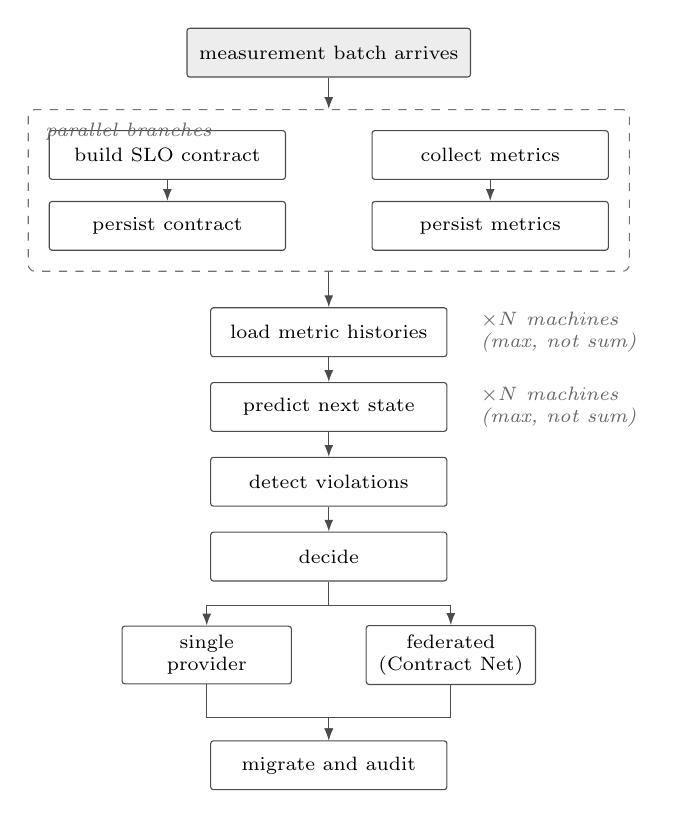
\begin{tikzpicture}[
    font=\scriptsize,
    st/.style  = {draw=black!70, rounded corners=1pt, minimum width=3.0cm,
                  minimum height=6.2mm, align=center, fill=white},
    stn/.style = {st, minimum width=2.15cm},
    trg/.style = {st, fill=black!7, minimum width=3.6cm},
    par/.style = {draw=black!55, dashed, rounded corners=2.5pt, inner sep=2.6mm},
    ar/.style  = {-{Latex[length=1.5mm]}, draw=black!70},
    ann/.style = {font=\scriptsize\itshape, text=black!60, align=left},
]

%--- trigger
\node[trg] (trig) at (0,0) {measurement batch arrives};

%--- parallel block: two independent branches
\node[st] (a1) at (-2.05,-1.30) {build SLO contract};
\node[st] (a2) at (-2.05,-2.20) {persist contract};
\node[st] (b1) at ( 2.05,-1.30) {collect metrics};
\node[st] (b2) at ( 2.05,-2.20) {persist metrics};

\node[par, fit=(a1)(a2)(b1)(b2)] (pbox) {};
\node[ann, anchor=north west] at ([xshift=1mm,yshift=-0.5mm]pbox.north west)
      {parallel branches};

%--- sequential chain
\node[st] (h) at (0,-3.55) {load metric histories};
\node[st] (p) at (0,-4.50) {predict next state};
\node[st] (v) at (0,-5.45) {detect violations};
\node[st] (d) at (0,-6.40) {decide};

%--- two decision paths
\node[stn] (m1) at (-1.55,-7.65) {single\\provider};
\node[stn] (m3) at ( 1.55,-7.65) {federated\\(Contract Net)};

\node[st] (act) at (0,-9.05) {migrate and audit};

%--- edges
\draw[ar] (trig.south) -- (pbox.north);
\draw[ar] (a1) -- (a2);
\draw[ar] (b1) -- (b2);
\draw[ar] (pbox.south) -- (h.north);
\draw[ar] (h) -- (p);
\draw[ar] (p) -- (v);
\draw[ar] (v) -- (d);

\draw[ar] (d.south) -- ++(0,-0.30) -| (m1.north);
\draw[ar] (d.south) -- ++(0,-0.30) -| (m3.north);

\draw[ar] (m1.south) |- ([yshift=-0.42cm]m1.south) -| (act.north);
\draw[ar] (m3.south) |- ([yshift=-0.42cm]m1.south) -| (act.north);

%--- annotations: the two kinds of parallelism
\node[ann, anchor=west] at ([xshift=3mm]h.east) {$\times N$ machines\\(max, not sum)};
\node[ann, anchor=west] at ([xshift=3mm]p.east) {$\times N$ machines\\(max, not sum)};

\end{tikzpicture}
}
\caption{The orchestration cycle. The two branches of the parallel block have
no mutual dependency; everything below it is strictly sequential because each
stage consumes the previous one's output. Stages marked $\times N$ run
concurrently across the candidate machines, so their cost is the slowest
machine rather than the sum---a distinction that matters when reading the
timing results of Section~\ref{sec:eval}.}
\label{fig:cycle}
\end{figure}

Fig.~\ref{fig:cycle} shows one cycle. This section describes its structure;
the mechanisms invoked at each stage are the subject of
Section~\ref{sec:method}.

\subsection{Trigger and mutual exclusion}

A cycle starts when a batch of QoS measurements arrives from the consumer,
never on a timer. Orchestration is therefore paced by the observed system
rather than by a clock, and the system does no work when nothing changes.

Cycles do not overlap. A batch that arrives while a cycle is in flight is
\emph{dropped}, not queued. This is a deliberate trade-off: under sustained
load some measurements are lost. We accept it because the alternative is
worse. A queue would make the orchestrator decide on observations that are
already stale by the time they are processed, and the staleness would grow
with the backlog---exactly the failure mode a proactive orchestrator exists to
avoid. Dropping keeps every decision anchored to the most recent view of the
system.

\subsection{Stages}

A cycle runs eight stages. It builds the SLO contract for the current
objective and persists it; it collects the QoS metrics of every candidate
machine and persists them; it loads the recent history of each metric;
it predicts the next value of each metric for each machine; it detects which
primary objectives are about to be breached; it decides where the service
should run; and, if the decision is to move, it applies the migration to the
infrastructure and records an audit trail.

The order is not a matter of style. From the history loading stage onward,
each stage consumes what the previous one produced---history feeds prediction,
prediction feeds detection, detection feeds the decision---so the chain admits
no reordering and no overlap.

\subsection{Two forms of parallelism}

The cycle exploits concurrency in two distinct ways, and the distinction is
what makes the measurements of Section~\ref{sec:eval} interpretable.

\emph{Independent branches.} Building the SLO contract and collecting metrics
have no mutual dependency: the contract derives from the objective and the
violation history, the metrics from the machines. They run as two concurrent
sequences, and only the stages below the block need both.

\emph{One stage across many machines.} Loading histories and predicting are
performed for every candidate machine at once. The cost of such a stage is the
duration of its \emph{slowest} machine, not the sum over machines.

Ignoring the second point is the classic way to misread a pipeline profile:
summing the per-machine durations yields a cycle time that never occurred. Our
instrumentation records, for every stage, whether its duration aggregates as a
sum or as a maximum, and Section~\ref{sec:eval} reports them accordingly.

A third source of latency is removed rather than parallelised. Querying the
machines over the network costs more than every other stage combined, so the
collection stage does not query them: a background poller keeps a fresh
snapshot, and the stage reads it. The network round-trip stays off the
critical path.

\subsection{Two decision paths}

The decision stage routes to one of two implementations, shown at the bottom
of Fig.~\ref{fig:cycle}.

\emph{Single-provider} ignores the federation entirely: TOPSIS ranks the local
compliant candidates and the best one wins.
\emph{Federated} runs the Contract Net round of
Section~\ref{sec:gap} whenever the incumbent's own primary objective is in
breach: broadcast, bids, arbitration, and either a local migration or an
award to the winning peer.

Routing is controlled by configuration, and the single-provider path is the
system's original code, untouched by the federation extension. This is what
makes the ablation of Section~\ref{sec:eval} meaningful: disabling the
federation does not approximate a federation-free system, it \emph{is} the
system as it existed before the extension, running the same contracts on the
same traces.

\section{Decision Mechanisms}
\label{sec:method}

This section presents the four mechanisms that turn an objective into a
placement. Each is introduced by the problem it solves, then formalised, then
justified against the alternatives, and finally illustrated on a single
21-minute run of the physical testbed described in
Section~\ref{sec:eval}. All figures quoted below are taken from that run's
logs; none is reconstructed.

\subsection{The chain, and why it has three links}
\label{sec:chain}

The mechanisms are not interchangeable, and the order in which they compose is
the argument of this section.

Mutual information \emph{widens} the contract: it adds the secondary metrics
that observation shows to accompany violations. TOPSIS \emph{ranks locally},
over the full criteria set---primary \emph{and} secondary---because inside one
provider the question is a trade-off between machines that all belong to the
same owner. The Gap Grade \emph{compares globally}, over the primary
objectives only, because across providers the question is no longer which
machine is preferable but whether the contract is met, and by how much.

This raises the obvious objection: if the Gap Grade is the only quantity that
crosses the boundary, why compute the other two at all? Three reasons, and
they are the reason the chain has three links rather than one.

First, the Gap Grade is deliberately \emph{blind to secondary objectives}. It
scores the contract, and only the operator's contract is contractual; a
metric that mutual information promoted is evidence, not a commitment. Ranking
candidates on it would let a discovered correlation override a stated goal.

Second, the Gap Grade is \emph{degenerate inside a pool}. Several machines of
one provider routinely satisfy the same primary objectives with similar
margins, and the Gap Grade cannot separate them: it measures distance to a
threshold, not the multi-criteria trade-off---latency against available cores
against available memory---that decides which of two compliant machines is the
better host. That is precisely what TOPSIS is for.

Third, running TOPSIS across the union of both pools would not fix the
problem, it would hide it: min--max normalisation over a merged pool produces
a ranking that depends on which machines happen to be present, so adding a
poor machine to one provider changes the score of a machine in the other. The
two questions are genuinely different, and each mechanism answers the one it
is valid for.

\begin{table}[t]
\centering
\caption{Testbed parameters used throughout this section. Latency is a
function of the distance between the vehicle and the target; the ranges below
are the extreme values of that mapping. Section~\ref{sec:eval} gives the full
setup.}
\label{tab:testbed-preview}
\footnotesize
\setlength{\tabcolsep}{4pt}
\begin{tabular}{@{}llrrl@{}}
\toprule
\textbf{Target} & \textbf{Provider} & \textbf{Cores} & \textbf{RAM}
& \textbf{Latency range}\\
\midrule
edge$_1$, edge$_2$       & P1, P2 & $2$  & $2$ GB  & \multirow{3}{*}{$5$--$150$ ms}\\
edge$_{1b}$, edge$_{2b}$ & P1, P2 & $3$  & $3$ GB  & \\
edge$_{1c}$, edge$_{2c}$ & P1, P2 & $4$  & $4$ GB  & \\
\addlinespace[2pt]
cloud$_1$                & P1     & $16$ & $16$ GB & \multirow{2}{*}{$50$--$230$ ms}\\
cloud$_2$                & P2     & $8$  & $8$ GB  & \\
\bottomrule
\end{tabular}
\end{table}

Table~\ref{tab:testbed-preview} summarises the testbed parameters the examples
below depend on. Two of them carry most of the explanatory weight: no edge
target exceeds $4$~GB of memory, and no cloud target can go below $50$~ms of
latency however close the vehicle comes. Both are properties of the
infrastructure, not of the orchestrator, and both will make the outcomes below
arithmetic rather than fortunate.

\subsection{From intent to a weighted contract}
\label{sec:intent}

\textbf{The problem.} The operator states a goal in natural language. The
orchestrator needs numeric thresholds, a weight per objective, and a rule for
combining the new objective with whatever contract is already active. Nothing
in the sentence supplies any of the three.

\textbf{The mechanism.} An LLM is prompted to identify the \emph{class of
service} that would fulfil the intention, and then to derive that class's QoS
needs. The same inference assigns each objective a weight in $[0,1]$ and
selects a merge strategy---\textsc{replace} when the new intention supersedes
the active contract, \textsc{additive} when it refines it. The model runs at
temperature $0$. Its output crosses a validation stage that checks the schema,
bounds each threshold to the range declared for its metric, and rejects any
objective naming an unknown metric. Non-determinism therefore stops at that
boundary: everything downstream consumes a contract that is structurally
valid by construction.

\textbf{Why not keyword extraction.} Consider the first intention of
Table~\ref{tab:intents}. It contains no metric name, no number, and no
technical term that maps onto CPU or memory. A keyword matcher has nothing to
match. What produces the contract is the inference \emph{4K upscaling and
multi-angle reconstruction is a compute-bound service}, followed by the
derivation of what such a service needs. This is a modelling step, not a
parsing step, which is why a language model earns its place here.

\begin{table}[t]
\centering
\caption{The two intentions of the run and the contracts they produced.
Neither sentence contains a metric name or a number.}
\label{tab:intents}
\footnotesize
\setlength{\tabcolsep}{4pt}
\begin{tabularx}{\columnwidth}{@{}X@{}}
\toprule
\textbf{\emph{``Enable AI-based 4K upscaling and multi-angle scene
reconstruction on my stream, I need maximum compute power''}}\\[2pt]
$\rightarrow$ \texttt{cpu\_usage} $\geq 4$ cores \quad (weight $0.60$,
primary)\\
$\rightarrow$ \texttt{ram\_usage} $\geq 8$ GB \quad\ (weight $0.40$,
primary)\\
\emph{latency is removed from the contract} --- strategy \textsc{replace}\\
\midrule
\textbf{\emph{``Reduce latency as much as possible, I'm watching a live
event''}}\\[2pt]
$\rightarrow$ \texttt{latency} $< 50$ ms \quad (weight $1.00$, primary)\\
\emph{compute objectives removed} --- strategy \textsc{replace}\\
\bottomrule
\end{tabularx}
\end{table}

\textbf{On the run.} The first intention produced a contract with \emph{no
latency objective at all}. Its consequence is arithmetic rather than
editorial: the most capable edge machine in the testbed offers 4 cores but
only 4~GB of memory, so it satisfies the CPU objective and fails the memory
one---no edge target is a candidate at either provider. Only cloud-class
capacity clears both bounds, and which of the two cloud targets ends up
hosting the service is not fixed by raw capacity: the larger machine does not
always carry the larger \emph{available} margin, since availability tracks
current load rather than provisioned size. At one recorded handover, the
second provider's own champion failed to clear the memory bound under its
measured load (\texttt{champion=None}, \texttt{conforme=False} in the
deployment log), leaving the first provider's cloud target the sole compliant
bid; the arbiter's log records a single retained bid, not a comparison
between two. The LLM did not ``choose the cloud''; it produced a contract
that only cloud-class capacity can satisfy, and from one instant to the next,
either target can be the one left standing.

The second intention set a $50$~ms latency bound. In this testbed the cloud
targets cannot go below $50$~ms by construction (Section~\ref{sec:eval}), so
they are excluded by a strict inequality, and the service returned to the
edge---this time to an edge target belonging to the \emph{other} provider.

\subsection{Self-supervised contract enrichment}
\label{sec:mi}

\textbf{The problem.} A contract states what the operator asked for. It says
nothing about the quantities that happen to accompany violations on this
infrastructure. Those quantities are worth watching, and nobody has declared
them.

\textbf{The mechanism.} Let $X$ be an observed metric and $Y \in \{0,1\}$ the
violation signal of the primary objectives. The system estimates the mutual
information
\begin{equation}
I(X;Y) = H(X) - H(X \mid Y),
\label{eq:mi}
\end{equation}
normalised by $H(Y)$ so that the score lies in $[0,1]$. Differential entropies
are estimated with a $k$-nearest-neighbour
estimator~\cite{kraskov2004}: for $n$ samples and the distance $r_k$ to the
$k$-th neighbour,
\begin{equation}
\hat{H}(X) \simeq \psi(n) - \psi(k) + \ln 2 + \frac{1}{n}\sum_{i=1}^{n} \ln r_{k,i},
\label{eq:kl}
\end{equation}
where $\psi$ is the digamma function. A metric whose normalised score exceeds
a relative threshold becomes a \emph{secondary} objective, and---this is the
point---its weight \emph{is} its score. Primary thresholds are never
recomputed; only the periphery of the contract moves.

The series feeding Eq.~\eqref{eq:mi} is that of the target \emph{currently
hosting the service}, not a per-candidate or pooled history. The contract is
therefore learned from the path actually served, which is the only path on
which a violation has an observable meaning. A consequence follows for the
federation: a \textsc{standby} provider hosts nothing, so it computes no
score and keeps the contract it adopted from the initiator---which is also
what guarantees that both providers negotiate on identical terms.

\textbf{Why mutual information, and why this estimator.} Three properties
decide the choice. Mutual information detects arbitrary dependence, whereas a
Pearson correlation sees only the linear part; on a saturating resource, the
relationship of interest is precisely the non-linear one. Estimating it by
binning the values would make the result depend on a bin count nobody can
justify, and would discard information inside each bin; the $k$-NN estimator
works on the continuous values directly and is usable from roughly fifteen
samples per class, which matters because $Y=1$ is by design a rare event.
Finally, using the score itself as the weight removes a free parameter: a
metric that explains violations twice as well counts twice as much, and no
constant needs to be tuned.

\textbf{On the run.} Table~\ref{tab:mi} shows the contract over three
consecutive estimations, forty seconds apart. The primary threshold is
untouched throughout; what moves is which metrics accompany it and how much
they weigh.

\begin{table}[t]
\centering
\caption{Contract enrichment by mutual information over three consecutive
estimations. The primary threshold never changes; secondary objectives appear,
disappear, and are weighted by their own score.}
\label{tab:mi}
\scriptsize
\setlength{\tabcolsep}{4pt}
\begin{tabular}{@{}llll@{}}
\toprule
\textbf{Time} & \textbf{Primary} & \textbf{Secondary} & \textbf{Weights}\\
\midrule
14:21:09 & \texttt{lat} $<28$ ms & \texttt{cpu} & $0.65$ / $0.35$\\
14:21:21 & \texttt{lat} $<28$ ms & \texttt{cpu}, \texttt{ram}
         & $0.54$ / $0.26$ / $0.20$\\
14:21:45 & \texttt{lat} $<28$ ms & \texttt{cpu} & $0.84$ / $0.16$\\
\bottomrule
\end{tabular}

\vspace{2pt}
{\scriptsize \texttt{lat}, \texttt{cpu}, \texttt{ram} abbreviate
\texttt{latency}, \texttt{cpu\_usage}, \texttt{ram\_usage}.}
\end{table}

\textbf{What a wrong score can and cannot do.} Because the estimate is
statistical, the bound on its consequences matters. A secondary objective is
a \emph{weight}, never a \emph{constraint}: it enters neither the compliance
filter (Section~\ref{sec:topsis}) nor the Gap Grade
(Section~\ref{sec:gap}), both computed on the primary objectives alone. A
spurious dependency can therefore reorder candidates that already satisfy the
contract, but it can neither produce a non-compliant placement nor alter an
inter-provider verdict---it degrades the quality of a choice, never its
validity. Section~\ref{sec:limit-mi} shows that this bound is load-bearing on
our testbed.

Two further observations follow. The contract is re-estimated every cycle and
is not smoothed, so secondary weights move substantially between consecutive
estimations---we return to this in Section~\ref{sec:discussion}. And the
mechanism is structurally dependent on violations existing: with no violation
in the recent history, every score is zero and the contract stays bare. It is
richer under stress than at rest, which is inherent to a supervised measure of
dependence.

\subsection{Ranking inside a provider: TOPSIS}
\label{sec:topsis}

\textbf{The problem.} Given a contract and a set of candidate targets, rank
them on criteria that conflict with one another and are expressed in
incompatible units---milliseconds, percentages, cores, gigabytes.

\textbf{The mechanism.} Candidates are first filtered: a target predicted to
violate a \emph{primary} objective is removed outright, whatever its other
qualities. The survivors enter TOPSIS~\cite{hwang1981} in four phases, over
the $n$ compliant candidates and the $m$ criteria of the contract---primary
and secondary alike.

\emph{Phase 1 --- decision matrix.} The matrix $X = [x_{ij}]$ is built on the
\emph{predicted} value of criterion $j$ for candidate $i$, never on the
measured one. Resource criteria enter through the capacity conversion of
Eq.~\eqref{eq:capacity} below.

\emph{Phases 2 and 3 --- normalisation and weighting.} Each column is
min--max normalised onto $[0,1]$ with its orientation, so that $1$ always
denotes the most desirable value, then scaled by the weight the contract
carries for that criterion---an LLM-assigned weight for a primary objective,
a mutual-information score for a secondary one:
\begin{equation}
v_{ij} = w_j \, r_{ij}, \qquad \textstyle\sum_j w_j = 1 .
\label{eq:weight}
\end{equation}

\emph{Phase 4 --- ideal solutions and closeness.} The ideal $A^{+}$ and
anti-ideal $A^{-}$ are the best and worst weighted value of each criterion,
$v_j^{+} = \max_i v_{ij}$ and $v_j^{-} = \min_i v_{ij}$. Each candidate is
scored by its relative closeness to $A^{+}$:
\begin{equation}
C_i = \frac{d_i^{-}}{d_i^{+} + d_i^{-}}, \qquad
d_i^{\pm} = \sqrt{\textstyle\sum_{j=1}^{m} \left(v_{ij} - v_j^{\pm}\right)^2 }.
\label{eq:topsis}
\end{equation}
The elected candidate maximises $C_i \in [0,1]$.

The phases are printed as tables at run time, which makes any decision
recomputable by hand from the log---the explainability requirement of
Section~\ref{sec:intro} is met by construction rather than by a summary.

\textbf{Two properties specific to this implementation.} First, a
\emph{capacity conversion}. Resource usage enters the matrix not as a
percentage but as the absolute headroom it leaves:
\begin{equation}
a_{ij} = C_j \times \left(1 - u_{ij}/100\right),
\label{eq:capacity}
\end{equation}
where $C_j$ is the capacity the target declares for that resource. The
criterion then flips from cost to benefit. Without this conversion, two
targets at $50\%$ CPU are indistinguishable, although one may leave $1$ core
free and the other $8$. Capacity is declared by the target itself rather than
tabulated in the orchestrator, so adding a machine requires no change to the
decision code.

Second, a \emph{tie guard}. A criterion whose relative spread across the
candidates falls below $1\%$ is neutralised to $0.5$ for every candidate.
Min--max normalisation is scale-free, so without this guard $0.1$~ms of model
noise on values around $100$~ms is amplified into a full $0$-to-$1$ spread,
and a candidate can be assigned a closeness of exactly $0$---which silently
disables the multiplicative hysteresis that prevents oscillation.

\textbf{Why not a weighted sum.} A weighted sum lets a large advantage on one
criterion compensate an arbitrarily bad value on another. TOPSIS scores
distance to an ideal point, so a candidate that is extreme on one axis is
penalised for its distance on the others. We claim no novelty for TOPSIS
itself; it is a standard and appropriate tool for this sub-problem, and the
contribution lies in what surrounds it---the capacity conversion above, and
the boundary of its validity established next.

\textbf{On the run.} Table~\ref{tab:matrix} gives a real decision matrix, for
provider~2 at the cycle that immediately preceded the second intention's
migration. The capacity conversion is visible: the cloud target is the worst
candidate on latency and by far the best on available resources, while the
edge targets are the reverse. Under the active contract---latency below
$50$~ms---the compliance filter retains a single candidate, and TOPSIS is
therefore trivial at this instant. That is not a weakness of the method but a
property of a tight contract, and it is exactly why the interesting comparison
happens at the next level.

\begin{table}[t]
\centering
\caption{Decision matrix of provider~2, one cycle before the handover, on
predicted values. Available cores and memory are obtained from the predicted
usage by Eq.~\eqref{eq:capacity}. Under \texttt{latency} $<50$ ms, a single
candidate survives the compliance filter.}
\label{tab:matrix}
\footnotesize
\setlength{\tabcolsep}{4pt}
\begin{tabular}{@{}lrrrrrc@{}}
\toprule
\textbf{Target} & \textbf{lat.} & \textbf{CPU} & \textbf{avail.}
& \textbf{RAM} & \textbf{avail.} & \textbf{compl.}\\
 & (ms) & (\%) & (cores) & (\%) & (GB) & \\
\midrule
edge$_2$   & $71.1$ & $55.8$ & $0.88$ & $78.3$ & $0.43$ & --- \\
edge$_{2b}$ & $\mathbf{17.0}$ & $72.3$ & $0.83$ & $52.1$ & $1.44$
           & $\checkmark$ \\
edge$_{2c}$ & $68.0$ & $60.2$ & $1.59$ & $51.6$ & $1.94$ & --- \\
cloud$_2$  & $89.0$ & $10.2$ & $\mathbf{7.18}$ & $16.3$ & $\mathbf{6.70}$
           & --- \\
\bottomrule
\end{tabular}
\end{table}

\subsection{Comparing across providers: the Gap Grade}
\label{sec:gap}

\textbf{The problem.} Each provider has now ranked its own targets and holds a
champion with a closeness score. These two scores cannot be compared, and the
reason is structural rather than practical.

\textbf{Why TOPSIS stops at the provider boundary.} Min--max normalisation is
relative to the set it is applied to. The best candidate of \emph{any} set
maps to $1$ on every criterion where it leads, so the winner of a pool of
excellent machines and the winner of a pool of poor ones both score close to
$1$. A closeness of $0.98$ asserts \emph{best here}; it asserts nothing about
absolute quality. Selecting between providers by comparing closeness scores is
therefore not an approximation---it is meaningless.
Fig.~\ref{fig:twoscales} makes the point visually.

\begin{figure}[t]
\centering
\resizebox{\columnwidth}{!}{% Figure 3 --- why a pool-relative score cannot cross a provider boundary,
% and what replaces it. Values are those of the run of Section V.
% Included from paper.tex.

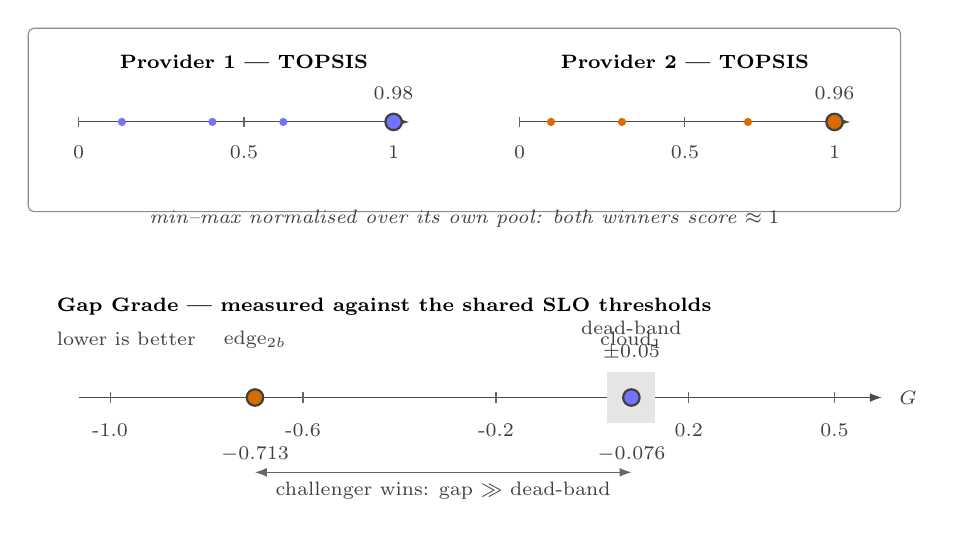
\begin{tikzpicture}[
    font=\scriptsize,
    ax/.style   = {-{Latex[length=1.5mm]}, draw=black!70},
    tick/.style = {draw=black!60},
    p1/.style   = {circle, fill=blue!55, inner sep=1.05pt},
    p2/.style   = {circle, fill=orange!85!black, inner sep=1.05pt},
    win/.style  = {circle, draw=black!75, thick, inner sep=2.1pt},
    lbl/.style  = {font=\scriptsize, text=black!75},
    box/.style  = {draw=black!45, rounded corners=2pt, inner sep=2.4mm},
]

%======== TOP: two pool-relative TOPSIS axes ========
% --- Provider 1
\draw[ax] (0,0) -- (4.2,0);
\foreach \x/\t in {0/0, 2.1/0.5, 4.0/1} \draw[tick] (\x,-0.6mm) -- (\x,0.6mm)
    node[below=1.2mm, lbl] at (\x,-0.6mm) {\t};
\node[p1] at (0.55,0) {};
\node[p1] at (1.70,0) {};
\node[p1] at (2.60,0) {};
\node[p1, win] (w1) at (4.00,0) {};
\node[lbl, above=1.6mm] at (4.00,0) {$0.98$};
\node[font=\scriptsize\bfseries, above=5.5mm] at (2.1,0) {Provider 1 --- TOPSIS};

% --- Provider 2
\begin{scope}[xshift=5.6cm]
\draw[ax] (0,0) -- (4.2,0);
\foreach \x/\t in {0/0, 2.1/0.5, 4.0/1} \draw[tick] (\x,-0.6mm) -- (\x,0.6mm)
    node[below=1.2mm, lbl] at (\x,-0.6mm) {\t};
\node[p2] at (0.40,0) {};
\node[p2] at (1.30,0) {};
\node[p2] at (2.90,0) {};
\node[p2, win] (w2) at (4.00,0) {};
\node[lbl, above=1.6mm] at (4.00,0) {$0.96$};
\node[font=\scriptsize\bfseries, above=5.5mm] at (2.1,0) {Provider 2 --- TOPSIS};
\end{scope}

\node[box, fit={(-0.4,-0.9) (10.2,0.95)}] (topbox) {};
\node[lbl, anchor=north] at (4.9,-1.0)
  {\itshape min--max normalised over its own pool: both winners score $\approx 1$};

%======== BOTTOM: one absolute Gap Grade axis ========
\begin{scope}[yshift=-3.5cm]
\draw[ax] (0,0) -- (10.2,0);
\node[lbl, anchor=west] at (10.3,0) {$G$};

\foreach \x/\t in {0.4/-1.0, 2.85/-0.6, 5.30/-0.2, 7.75/0.2, 9.6/0.5}
    \draw[tick] (\x,-0.7mm) -- (\x,0.7mm) node[below=1.4mm, lbl] at (\x,-0.7mm) {\t};

% dead-band around the incumbent (provider 1)
\fill[black!10] (6.71,-0.32) rectangle (7.32,0.32);
\node[lbl, anchor=south, align=center] at (7.02,0.36) {dead-band\\$\pm 0.05$};

\node[p2, win] (g2) at (2.24,0) {};
\node[lbl, anchor=south] at (2.24,0.5) {edge$_{2b}$};
\node[lbl, anchor=north] at (2.24,-0.5) {$-0.713$};

\node[p1, win] (g1) at (7.02,0) {};
\node[lbl, anchor=south] at (7.02,0.5) {cloud$_1$};
\node[lbl, anchor=north] at (7.02,-0.5) {$-0.076$};

\draw[{Latex[length=1.5mm]}-{Latex[length=1.5mm]}, draw=black!60]
      (2.24,-0.95) -- node[below, lbl] {challenger wins: gap $\gg$ dead-band} (7.02,-0.95);

\node[font=\scriptsize\bfseries, anchor=west] at (-0.4,1.15)
  {Gap Grade --- measured against the shared SLO thresholds};
\node[lbl, anchor=west] at (-0.4,0.75) {lower is better};
\end{scope}

\end{tikzpicture}
}
\caption{The two scales. Above, each provider normalises over its own pool, so
both champions land near $1$ regardless of absolute quality---the scores are
not comparable. Below, the Gap Grade places the same two champions on a single
axis defined by the shared SLO thresholds, where the distance between them is
meaningful. Values are those of the handover discussed in the text.}
\label{fig:twoscales}
\end{figure}

\textbf{The mechanism.} Comparison uses a quantity measured against the
thresholds themselves. For each \emph{primary} objective $i$ with threshold
$\tau_i$ and predicted value $v_i$, define the relative shortfall
\begin{equation}
\delta_i =
\begin{cases}
(v_i - \tau_i)/\tau_i & \text{cost objective } (v_i < \tau_i \text{ desired}),\\
(\tau_i - v_i)/\tau_i & \text{benefit objective},
\end{cases}
\label{eq:delta}
\end{equation}
floored at $-1$. The Gap Grade aggregates the $\delta_i$ by an augmented
Tchebycheff scalarisation~\cite{steuer1983}:
\begin{equation}
G = \frac{\max_i \left(w_i\,\delta_i\right) \;+\; \rho \sum_i w_i\,\delta_i}
         {1 + \rho}, \qquad \rho = 0.1 .
\label{eq:gapgrade}
\end{equation}
$G$ is negative when the contract is met with margin, positive when it is
breached, and \emph{lower is better}---the opposite polarity to TOPSIS
closeness. The two are never combined.

\textbf{Why an augmented Tchebycheff form.} The $\max$ term makes the measure
pessimistic: a provider is judged on its worst weighted objective, so it
cannot hide one breached metric behind several comfortable ones. A plain
weighted sum would allow exactly that compensation, which is unacceptable when
the objectives are contractual. The small $\rho \sum_i$ term breaks ties
between providers whose worst objective coincides, and keeps the measure
strictly monotone. Because every $\delta_i$ is expressed relative to a
threshold both providers share, $G$ carries the same meaning in both domains
--- which is the entire requirement.

\textbf{Arbitration.} The provider that detects the violation becomes the
\emph{initiator} of a Contract Net round~\cite{smith1980}: it broadcasts the
complete contract, builds its own bid in parallel, collects the peers' bids,
and submits all of them to an arbiter. Initiator is a role attached to an
event, not a standing coordinator, so any provider may hold it. The arbiter
selects the lowest $G$, but displaces the incumbent only if the improvement
exceeds an absolute dead-band---without it, two providers whose Gap Grades
straddle each other by noise would exchange the service indefinitely.

\textbf{On the run.} At the handover of Section~\ref{sec:intent}, the
arbiter recorded:

\begin{quote}\itshape\footnotesize
provider-2 takes the service on edge$_{2b}$ ($-0.7130$): beats provider-1
($-0.0760$) beyond the dead-band $0.0500$.
\end{quote}

Both numbers are on the same axis, and the decision reads directly from
Eq.~\eqref{eq:gapgrade}: with a single primary objective of weight $1$ and a
threshold of $50$~ms, a predicted latency of about $14.7$~ms gives
$\delta = (14.7 - 50)/50 \simeq -0.71$, and $G = \delta$ since the $\max$ and
the sum coincide. The challenger's margin is an order of magnitude larger than
the incumbent's, and the dead-band is cleared without ambiguity.

Two of the six handovers of the run ended the other way---\emph{provider-1
keeps the service on cloud$_1$: already the best Gap Grade}. The protocol runs
on every detected violation; it concludes in a move only when the absolute
evidence supports one.

At the limit, this holds even when two bids are numerically identical.
Ranking two candidates with equal Gap Grades can place either one first, but
the outcome is unaffected: the incumbent is displaced only when the challenger
clears the dead-band (\texttt{best\_gap < incumbent\_gap - deadband}), and an
exact tie never satisfies a strict inequality. Two targets belonging to
different providers with identical predicted latency therefore never trade
the service back and forth---the incumbent keeps it, regardless of which
provider's bid a tie-break would otherwise favour.

\section{Evaluation}
\label{sec:eval}
\subsection{Experimental protocol}
\label{sec:protocol}

Three conditions are evaluated on the testbed of
Table~\ref{tab:testbed-preview}. \textbf{Federated} runs the complete system
with both providers active. \textbf{Ablated} runs the same code, on the same
trajectory, with the federation disabled: a single orchestrator, four
placement targets, no negotiation. This is an ablation in the strict sense---
one variable changes, and the contract, threshold, cycle period and decision
code are identical. \textbf{Static} is the placement a latency-agnostic
scheduler produces: the service is placed once and never moved. We derive it
analytically from the trajectory rather than measuring it, and report it for
every possible fixed choice, so no assumption is made about which target such
a scheduler would pick.

Each condition was executed \textbf{four times}, on separate days, with the
infrastructure restarted between runs. No code changed between the eight
executions. The measurement window of a run is the
interval over which its orchestrator was active, recovered from the timing
logs rather than declared, and ranges from $40.5$ to $108.4$~min across the
eight runs. The reported metric is a \emph{share} of trajectory samples, so
unequal durations need no rescaling; trajectory samples falling outside a
run's window---the vehicle occasionally circulates before the orchestrator
starts---are discarded rather than attributed to a target the system had no
opportunity to choose.

Violation is measured on \emph{ground truth}, not on the orchestrator's
beliefs. For every trajectory sample we recover which target actually hosted
the service at that instant, read that target's \emph{measured} latency, and
count the sample as violating when it exceeds the primary threshold of
28\,ms. Prediction quality is evaluated separately
(Section~\ref{sec:mlacc}); it never enters the violation figure.

Fig.~\ref{fig:trajectory} shows why the problem is non-trivial. Inverting the
distance-to-latency mapping at the $28$\,ms threshold gives a compliance
radius of $15.2$\,cm around an edge target. The consumer's path leaves those
discs for much of the lap, and the two cloud targets---whose latency floor of
$50$\,ms exceeds the threshold---never contribute a compliant region at all.
No orchestrator can serve within contract outside the shaded areas.

\begin{figure}[t]
\centering
\resizebox{0.92\columnwidth}{!}{% Figure 4 --- trajectoire du consommateur et couverture des cibles.
% Genere depuis data_UC1_federe/latences_session.csv (donnees reelles).
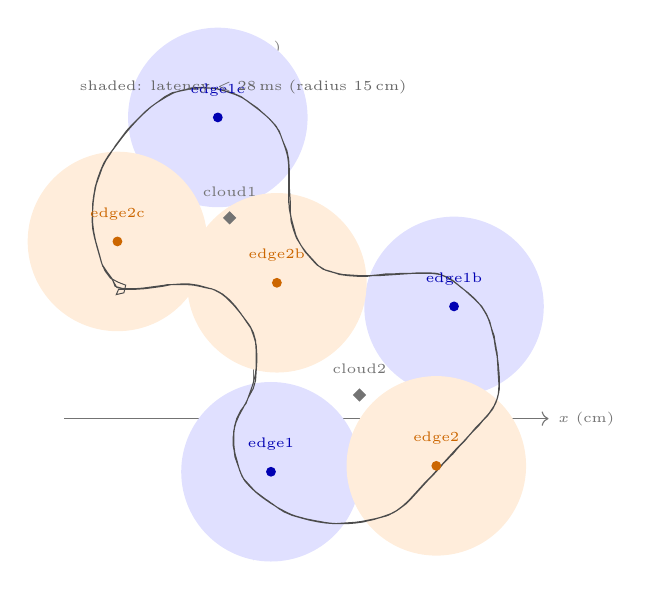
\begin{tikzpicture}[font=\scriptsize, scale=0.075]
  \draw[->,black!55] (-32,0) -- (50,0) node[right,font=\tiny]{$x$ (cm)};
  \draw[->,black!55] (0,-24) -- (0,60) node[above,font=\tiny]{$y$ (cm)};
  \fill[blue!12] (3,-9) circle (15.2);
  \fill[blue!12] (34,19) circle (15.2);
  \fill[blue!12] (-6,51) circle (15.2);
  \fill[orange!14] (31,-8) circle (15.2);
  \fill[orange!14] (4,23) circle (15.2);
  \fill[orange!14] (-23,30) circle (15.2);
  \draw[black!70, line width=0.35pt] (-1.7,1.8) -- (-1.7,1.8) -- (-2.3,0.8) -- (-2.9,-0.6) -- (-3.3,-2.0) -- (-3.4,-3.5) -- (-3.3,-5.0) -- (-3.1,-6.5) -- (-2.6,-7.9) -- (-2.1,-9.3) -- (-1.4,-10.6) -- (-0.4,-11.7) -- (0.7,-12.7) -- (1.9,-13.6) -- (3.2,-14.4) -- (4.4,-15.3) -- (5.8,-16.0) -- (7.2,-16.5) -- (8.6,-16.9) -- (10.1,-17.2) -- (11.6,-17.5) -- (13.0,-17.7) -- (14.5,-17.8) -- (16.0,-17.8) -- (17.5,-17.6) -- (19.0,-17.4) -- (20.4,-17.1) -- (21.9,-16.6) -- (23.3,-16.1) -- (24.6,-15.4) -- (25.8,-14.5) -- (26.9,-13.4) -- (27.9,-12.3) -- (28.9,-11.2) -- (29.9,-10.1) -- (30.9,-9.0) -- (31.9,-7.9) -- (33.0,-6.8) -- (34.0,-5.7) -- (35.0,-4.6) -- (36.0,-3.5) -- (37.0,-2.4) -- (38.1,-1.3) -- (39.0,-0.2) -- (40.0,1.0) -- (40.8,2.2) -- (41.4,3.6) -- (41.7,5.1) -- (41.7,6.6) -- (41.6,8.1) -- (41.4,9.6) -- (41.3,11.1) -- (41.0,12.5) -- (40.8,14.0) -- (40.3,15.4) -- (39.8,16.9) -- (39.2,18.2) -- (38.3,19.4) -- (37.3,20.5) -- (36.1,21.5) -- (35.0,22.4) -- (33.8,23.4) -- (32.5,24.1) -- (31.1,24.6) -- (29.6,24.7) -- (28.1,24.7) -- (26.6,24.6) -- (25.1,24.6) -- (23.6,24.5) -- (22.1,24.4) -- (20.6,24.3) -- (19.1,24.1) -- (17.6,24.1) -- (16.1,24.2) -- (14.6,24.4) -- (13.2,24.9) -- (11.8,25.3) -- (10.6,26.2) -- (9.6,27.3) -- (8.6,28.5) -- (7.8,29.8) -- (7.2,31.1) -- (6.8,32.6) -- (6.4,34.0) -- (6.1,35.5) -- (6.0,37.0) -- (6.0,38.5) -- (6.0,40.0) -- (6.0,41.5) -- (6.0,43.0) -- (5.8,44.5) -- (5.4,45.9) -- (4.9,47.3) -- (4.4,48.7) -- (3.5,49.9) -- (2.5,51.0) -- (1.3,52.0) -- (0.2,52.9) -- (-1.0,53.8) -- (-2.3,54.6) -- (-3.7,55.2) -- (-5.1,55.6) -- (-6.6,55.9) -- (-8.1,56.0) -- (-9.6,56.0) -- (-11.1,55.8) -- (-12.5,55.5) -- (-13.9,55.0) -- (-15.2,54.3) -- (-16.5,53.4) -- (-17.7,52.5) -- (-18.7,51.5) -- (-19.8,50.4) -- (-20.8,49.3) -- (-21.8,48.1) -- (-22.7,47.0) -- (-23.6,45.8) -- (-24.5,44.6) -- (-25.3,43.3) -- (-25.9,41.9) -- (-26.4,40.5) -- (-26.8,39.1) -- (-27.0,37.6) -- (-27.2,36.1) -- (-27.2,34.6) -- (-27.2,33.1) -- (-27.0,31.6) -- (-26.7,30.1) -- (-26.3,28.7) -- (-25.9,27.2) -- (-25.5,25.8) -- (-24.6,24.6) -- (-23.8,23.4) -- (-23.1,22.2) -- (-21.7,22.0) -- (-20.1,22.0) -- (-18.7,22.1) -- (-17.2,22.3) -- (-15.7,22.5) -- (-14.2,22.7) -- (-12.7,22.7) -- (-11.2,22.7) -- (-9.7,22.6) -- (-8.3,22.2) -- (-6.8,21.9) -- (-5.5,21.2) -- (-4.3,20.3) -- (-3.3,19.2) -- (-2.3,18.0) -- (-1.4,16.8) -- (-0.5,15.6) -- (0.1,14.3) -- (0.4,12.8) -- (0.5,11.3) -- (0.5,9.8) -- (0.5,8.3) -- (0.2,6.8) -- (-0.2,5.4) -- (-0.7,4.0) -- (-1.2,2.6) -- (-2.1,1.4) -- (-2.8,0.0) -- (-3.2,-1.4) -- (-3.3,-2.9) -- (-3.3,-4.4) -- (-3.1,-5.9) -- (-2.7,-7.3) -- (-2.3,-8.8) -- (-1.7,-10.1) -- (-0.7,-11.2) -- (0.3,-12.3) -- (1.5,-13.2) -- (2.7,-14.1) -- (4.0,-15.0) -- (5.2,-15.8) -- (6.6,-16.4) -- (8.0,-16.8) -- (9.5,-17.2) -- (11.0,-17.5) -- (12.4,-17.7) -- (13.9,-17.8) -- (15.4,-17.7) -- (16.9,-17.6) -- (18.4,-17.4) -- (19.9,-17.1) -- (21.4,-16.8) -- (22.8,-16.4) -- (24.1,-15.7) -- (25.3,-14.8) -- (26.4,-13.8) -- (27.4,-12.7) -- (28.4,-11.6) -- (29.5,-10.5) -- (30.5,-9.4) -- (31.5,-8.3) -- (32.5,-7.2) -- (33.5,-6.1) -- (34.6,-5.0) -- (35.6,-3.9) -- (36.6,-2.8) -- (37.6,-1.6) -- (38.6,-0.6) -- (39.7,0.5) -- (40.6,1.7) -- (41.2,3.0) -- (41.6,4.5) -- (41.6,6.0) -- (41.5,7.5) -- (41.4,9.0) -- (41.3,10.5) -- (41.0,12.0) -- (40.8,13.4) -- (40.4,14.9) -- (40.1,16.3) -- (39.5,17.7) -- (38.7,19.0) -- (37.6,20.1) -- (36.5,21.1) -- (35.4,22.1) -- (34.2,23.0) -- (33.0,23.9) -- (31.6,24.4) -- (30.2,24.6) -- (28.7,24.6) -- (27.2,24.6) -- (25.7,24.5) -- (24.2,24.4) -- (22.7,24.3) -- (21.2,24.2) -- (19.7,24.2) -- (18.2,24.2) -- (16.7,24.3) -- (15.2,24.4) -- (13.7,24.7) -- (12.3,25.1) -- (11.0,25.9) -- (10.0,27.0) -- (9.0,28.1) -- (8.1,29.3) -- (7.3,30.6) -- (6.8,32.0) -- (6.4,33.4) -- (6.3,34.9) -- (6.3,36.4) -- (6.2,37.9) -- (6.1,39.4) -- (6.1,40.9) -- (6.1,42.4) -- (6.0,43.9) -- (5.7,45.4) -- (5.1,46.8) -- (4.6,48.1) -- (3.9,49.5) -- (2.9,50.6) -- (1.8,51.6) -- (0.7,52.6) -- (-0.6,53.5) -- (-1.8,54.3) -- (-3.1,54.9) -- (-4.6,55.4) -- (-6.0,55.8) -- (-7.5,56.0) -- (-9.0,56.1) -- (-10.5,56.0) -- (-11.9,55.6) -- (-13.4,55.2) -- (-14.7,54.5) -- (-16.0,53.7) -- (-17.2,52.9) -- (-18.4,51.9) -- (-19.4,50.9) -- (-20.5,49.8) -- (-21.5,48.7) -- (-22.4,47.5) -- (-23.3,46.3) -- (-24.1,45.0) -- (-24.9,43.8) -- (-25.6,42.4) -- (-26.1,41.0) -- (-26.6,39.6) -- (-26.9,38.1) -- (-27.1,36.6) -- (-27.2,35.1) -- (-27.3,33.6) -- (-27.2,32.2) -- (-26.9,30.7) -- (-26.5,29.2) -- (-26.1,27.8) -- (-25.7,26.4) -- (-25.1,25.0) -- (-24.2,23.8) -- (-22.9,23.1) -- (-21.6,22.6) -- (-21.9,21.3) -- (-23.2,21.0) -- (-22.8,21.9) -- (-21.3,21.9) -- (-19.8,21.9) -- (-18.3,22.0) -- (-16.8,22.2) -- (-15.3,22.4) -- (-13.8,22.7) -- (-12.3,22.8) -- (-10.8,22.8) -- (-9.4,22.6) -- (-7.9,22.2) -- (-6.5,21.8) -- (-5.2,21.1) -- (-4.0,20.1) -- (-3.0,19.0) -- (-2.1,17.8) -- (-1.3,16.6) -- (-0.4,15.3) -- (0.1,13.9) -- (0.5,12.5) -- (0.6,11.0) -- (0.6,9.5) -- (0.5,8.0) -- (0.4,6.5) -- (-0.0,5.1) -- (-0.7,3.8) -- (-1.4,2.4) -- (-2.1,1.1) -- (-2.8,-0.2) -- (-3.2,-1.7) -- (-3.4,-3.1) -- (-3.4,-4.6) -- (-3.1,-6.1) -- (-2.7,-7.6) -- (-2.2,-9.0) -- (-1.6,-10.3) -- (-0.6,-11.5) -- (0.5,-12.5) -- (1.6,-13.4) -- (2.9,-14.3) -- (4.2,-15.1) -- (5.5,-15.8) -- (6.8,-16.4) -- (8.3,-16.8) -- (9.7,-17.2) -- (11.2,-17.4) -- (12.7,-17.7) -- (14.2,-17.8) -- (15.7,-17.8) -- (17.2,-17.7) -- (18.7,-17.5) -- (20.1,-17.1) -- (21.6,-16.7) -- (23.0,-16.3) -- (24.3,-15.6) -- (25.5,-14.7) -- (26.6,-13.7) -- (27.6,-12.6) -- (28.6,-11.4) -- (29.7,-10.3) -- (30.7,-9.3) -- (31.7,-8.2) -- (32.7,-7.0) -- (33.8,-6.0) -- (34.8,-4.8) -- (35.8,-3.8) -- (36.8,-2.6) -- (37.8,-1.6) -- (38.8,-0.4) -- (39.8,0.7) -- (40.7,1.9) -- (41.3,3.3) -- (41.6,4.7) -- (41.7,6.2) -- (41.6,7.7) -- (41.5,9.2) -- (41.3,10.7) -- (41.1,12.2) -- (40.8,13.7) -- (40.4,15.1) -- (40.0,16.6) -- (39.3,17.9) -- (38.5,19.2) -- (37.5,20.3) -- (36.4,21.3) -- (35.2,22.2) -- (34.1,23.1) -- (32.8,23.9) -- (31.4,24.5) -- (29.9,24.7) -- (28.4,24.7) -- (26.9,24.6) -- (25.4,24.6) -- (23.9,24.5) -- (22.4,24.5) -- (20.9,24.3) -- (19.4,24.1) -- (17.9,24.1) -- (16.4,24.2) -- (15.0,24.4) -- (13.5,24.8) -- (12.1,25.2) -- (10.8,26.0) -- (9.8,27.1) -- (8.8,28.2) -- (8.0,29.5) -- (7.3,30.8) -- (6.9,32.2) -- (6.5,33.7) -- (6.2,35.1) -- (6.0,36.6) -- (6.0,38.1) -- (6.0,39.6) -- (6.0,41.1) -- (6.0,42.6) -- (5.9,44.1) -- (5.5,45.6) -- (5.0,47.0) -- (4.5,48.4) -- (3.7,49.7) -- (2.7,50.8) -- (1.6,51.8) -- (0.4,52.7) -- (-0.8,53.6) -- (-2.0,54.5) -- (-3.4,55.1) -- (-4.8,55.5) -- (-6.2,55.9) -- (-7.7,56.0) -- (-9.2,56.0) -- (-10.7,55.8) -- (-12.2,55.5) -- (-13.7,55.2) -- (-15.0,54.5) -- (-16.2,53.6) -- (-17.4,52.7) -- (-18.5,51.7) -- (-19.6,50.6) -- (-20.6,49.6) -- (-21.6,48.4) -- (-22.5,47.2) -- (-23.4,46.0) -- (-24.3,44.8) -- (-25.1,43.6) -- (-25.7,42.2) -- (-26.3,40.8) -- (-26.7,39.4) -- (-27.0,37.9) -- (-27.2,36.4) -- (-27.2,34.9) -- (-27.2,33.4) -- (-27.1,31.9) -- (-26.8,30.5) -- (-26.4,29.0) -- (-26.0,27.6) -- (-25.6,26.1) -- (-24.8,24.9) -- (-23.9,23.7) -- (-23.4,22.4) -- (-22.0,22.0) -- (-20.5,22.0) -- (-19.0,22.0) -- (-17.5,22.2) -- (-16.0,22.4) -- (-14.5,22.7) -- (-13.0,22.7) -- (-11.5,22.7) -- (-10.1,22.6) -- (-8.6,22.3) -- (-7.1,22.0) -- (-5.7,21.4) -- (-4.6,20.5) -- (-3.5,19.4) -- (-2.5,18.3) -- (-1.6,17.1) -- (-0.7,15.9) -- (-0.0,14.6) -- (0.4,13.2) -- (0.5,11.7) -- (0.5,10.2) -- (0.5,8.7) -- (0.3,7.2) -- (-0.1,5.7) -- (-0.6,4.3) -- (-1.1,2.9) -- (-1.9,1.6) -- (-2.6,0.3) -- (-3.1,-1.1) -- (-3.3,-2.5) -- (-3.3,-4.0) -- (-3.2,-5.5) -- (-2.8,-7.0) -- (-2.4,-8.4) -- (-1.9,-9.8) -- (-1.0,-11.0) -- (0.1,-12.1) -- (1.2,-13.1) -- (2.5,-13.9) -- (3.7,-14.8) -- (4.9,-15.6) -- (6.3,-16.2) -- (7.7,-16.7) -- (9.2,-17.1) -- (10.6,-17.4) -- (12.1,-17.6) -- (13.6,-17.8) -- (15.1,-17.7) -- (16.6,-17.6) -- (18.1,-17.5) -- (19.6,-17.2) -- (21.0,-16.9) -- (22.5,-16.5) -- (23.8,-15.9) -- (25.1,-15.0) -- (26.2,-14.0) -- (27.2,-12.9) -- (28.2,-11.8) -- (29.2,-10.7) -- (30.3,-9.6) -- (31.3,-8.5) -- (32.3,-7.4) -- (33.3,-6.3) -- (34.3,-5.2) -- (35.4,-4.1) -- (36.4,-3.0) -- (37.4,-1.9) -- (38.4,-0.8) -- (39.4,0.3) -- (40.4,1.4) -- (41.1,2.7) -- (41.5,4.2) -- (41.6,5.7) -- (41.5,7.2) -- (41.4,8.7);
  \node[circle, fill=blue!70!black, draw=blue!70!black, inner sep=1.1pt] at (3,-9) {};
  \node[font=\tiny, text=blue!70!black, anchor=south] at (3,-7) {edge1};
  \node[circle, fill=blue!70!black, draw=blue!70!black, inner sep=1.1pt] at (34,19) {};
  \node[font=\tiny, text=blue!70!black, anchor=south] at (34,21) {edge1b};
  \node[circle, fill=blue!70!black, draw=blue!70!black, inner sep=1.1pt] at (-6,51) {};
  \node[font=\tiny, text=blue!70!black, anchor=south] at (-6,53) {edge1c};
  \node[circle, fill=orange!80!black, draw=orange!80!black, inner sep=1.1pt] at (31,-8) {};
  \node[font=\tiny, text=orange!80!black, anchor=south] at (31,-6) {edge2};
  \node[circle, fill=orange!80!black, draw=orange!80!black, inner sep=1.1pt] at (4,23) {};
  \node[font=\tiny, text=orange!80!black, anchor=south] at (4,25) {edge2b};
  \node[circle, fill=orange!80!black, draw=orange!80!black, inner sep=1.1pt] at (-23,30) {};
  \node[font=\tiny, text=orange!80!black, anchor=south] at (-23,32) {edge2c};
  \node[diamond, fill=black!55, draw=black!55, inner sep=1.1pt] at (-4,34) {};
  \node[font=\tiny, text=black!55, anchor=south] at (-4,36) {cloud1};
  \node[diamond, fill=black!55, draw=black!55, inner sep=1.1pt] at (18,4) {};
  \node[font=\tiny, text=black!55, anchor=south] at (18,6) {cloud2};
  \node[font=\tiny,anchor=north west,text=black!60] at (-31,59)
    {shaded: latency $<28$\,ms (radius 15\,cm)};
\end{tikzpicture}
}
\caption{Consumer trajectory over the measured lap, with the eight placement
targets. Shaded discs mark where a target satisfies the $28$\,ms objective
($15.2$\,cm radius, obtained by inverting the distance-to-latency mapping).
Circles are edge targets, diamonds cloud targets; blue belongs to provider~1,
orange to provider~2. Cloud targets have no compliant region: their latency
floor is $50$\,ms.}
\label{fig:trajectory}
\end{figure}

\subsection{Federation reduces SLO violation}
\label{sec:violation}

Table~\ref{tab:violation} reports the outcome. Two reference points frame the
measured systems: the \emph{oracle}, which would select the best available
target at every instant and therefore bounds what any orchestrator can
achieve, and the \emph{static} placement, which represents doing nothing.

\begin{table}[t]
\centering
\caption{Share of the lap spent in SLO violation (\texttt{latency}
$\geq 28$\,ms), measured on the consumer's ground-truth latency towards the
target actually hosting the service. Four independent runs per condition;
oracle and static bounds are averaged over the same four runs.}
\label{tab:violation}
\footnotesize
\setlength{\tabcolsep}{4pt}
\begin{tabular}{@{}lrr@{}}
\toprule
& \textbf{Ablated} & \textbf{Federated}\\
& \textbf{(4 targets)} & \textbf{(8 targets)}\\
\midrule
Static placement, best case   & $83.2\%$ & $81.9\%$\\
Static placement, mean        & $88.3\%$ & $88.3\%$\\
\addlinespace[2pt]
\textbf{Measured system, mean of 4 runs} & $\mathbf{54.8\%}$ & $\mathbf{23.8\%}$\\
\quad individual runs         & $53.7,52.7,56.6,56.3\%$ & $19.9,25.9,29.3,20.2\%$\\
\quad standard deviation      & $1.9$\,pt & $4.6$\,pt\\
\addlinespace[2pt]
Oracle (lower bound)          & $53.1\%$ & $7.5\%$\\
\midrule
Samples (4 runs)              & $6\,160$ & $8\,177$\\
Migrations (4 runs)           & $16,29,72,55$ & $30,34,34,68$\\
\bottomrule
\end{tabular}
\end{table}

Enabling the federation reduces violation from $54.8\%$ to $23.8\%$ on
average, a drop of some $31$ points---the consumer is served within contract
about $2.3$ times more often. Against the best static placement the
improvement is larger still, $81.9\%$ down to $23.8\%$, a factor of about
three and a half; and a latency-agnostic scheduler that happens to select a
cloud target never satisfies the contract at all, since no cloud target can
go below $50$\,ms by construction.

Four executions per condition are enough to test the gap, not just describe
it. The ablated condition reproduces closely---a standard deviation of
$1.9$~points across four runs spanning five days---which is what one expects
of a system already pinned against its own optimum by coverage. The
federated condition varies more, $4.6$~points, as one expects when the
decision has more freedom; Section~\ref{sec:threats} notes that we did not
find a single cause for this spread; an early hypothesis involving cloud
excursions in one run failed to generalise to the other three, so we report
the dispersion without attributing it. A two-sided exact Mann--Whitney test on
the four measurements per condition rejects equality
($U=16$, $p=0.029$)---the smallest $p$-value attainable at this sample size,
since the four ablated values exceed all four federated ones without
overlap. This significance does not depend on the measurement window chosen:
restricting the comparison to samples recorded after the first ten minutes of
each run yields the same test statistic ($U=16$, $p=0.029$).

The absolute figures deserve a word. A residual $23.8\%$ is not a failure of
the orchestrator but a property of the testbed: as Fig.~\ref{fig:trajectory}
shows, the consumer regularly travels through regions no target covers. The
oracle quantifies exactly this---even a perfect orchestrator would violate
$7.5\%$ of the lap.

Fig.~\ref{fig:latency} shows the same result as a time series rather than an
aggregate, with all four runs of each condition superimposed. The ablated
condition spends long continuous stretches above the threshold, corresponding
to the parts of the lap where none of provider~1's four targets is in range;
the federated condition crosses the threshold more often but returns below it
quickly, because a target belonging to the other provider becomes available.
The runs of a condition track each other closely enough that the distinction
between conditions is visible without any aggregation, and the density of
overlap is itself a picture of the reproducibility the table reports as a
standard deviation.

\begin{figure}[t]
\centering
\resizebox{0.95\columnwidth}{!}{% Figure 5 --- latence subie par le consommateur au cours du tour.
% Huit runs reels : 4 federes (bleu) et 4 ablation (orange), meme style
% par bras -- la densite de recouvrement montre la reproductibilite.
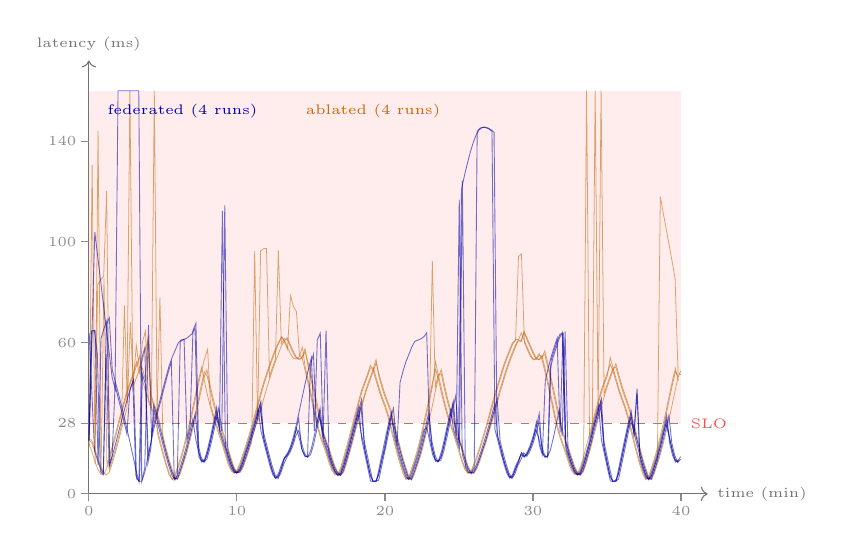
\begin{tikzpicture}[font=\scriptsize, xscale=0.188, yscale=0.032]
  \fill[red!7] (0,28.0) rectangle (40.0,160.0);
  \draw[->,black!55] (0,0) -- (41.8,0)    node[right,font=\tiny]{time (min)};
  \draw[->,black!55] (0,0) -- (0,172.0)    node[above,font=\tiny]{latency (ms)};
  \draw[black!45] (-0.5,0) -- (0,0) node[left,font=\tiny,xshift=-1pt]{0};
  \draw[black!45] (-0.5,28) -- (0,28) node[left,font=\tiny,xshift=-1pt]{28};
  \draw[black!45] (-0.5,60) -- (0,60) node[left,font=\tiny,xshift=-1pt]{60};
  \draw[black!45] (-0.5,100) -- (0,100) node[left,font=\tiny,xshift=-1pt]{100};
  \draw[black!45] (-0.5,140) -- (0,140) node[left,font=\tiny,xshift=-1pt]{140};
  \draw[black!45] (0,-3) -- (0,0) node[below,font=\tiny,yshift=-1pt]{0};
  \draw[black!45] (10,-3) -- (10,0) node[below,font=\tiny,yshift=-1pt]{10};
  \draw[black!45] (20,-3) -- (20,0) node[below,font=\tiny,yshift=-1pt]{20};
  \draw[black!45] (30,-3) -- (30,0) node[below,font=\tiny,yshift=-1pt]{30};
  \draw[black!45] (40,-3) -- (40,0) node[below,font=\tiny,yshift=-1pt]{40};
  \draw[red!65,dashed,line width=0.5pt] (0,28.0) -- (40.0,28.0)    node[right,font=\tiny,red!70]{SLO};
  \draw[orange!75!black, opacity=0.55, line width=0.28pt] (0.00,21.5) -- (0.17,21.5) -- (0.37,18.4) -- (0.57,14.9) -- (0.77,11.3) -- (0.97,8.8) -- (1.17,7.4) -- (1.37,8.6) -- (1.57,11.9) -- (1.77,15.9) -- (1.97,20.2) -- (2.17,24.9) -- (2.37,29.4) -- (2.57,33.8) -- (2.77,160.0) -- (2.97,42.1) -- (3.17,45.4) -- (3.37,48.6) -- (3.57,52.4) -- (3.77,56.4) -- (3.97,60.6) -- (4.17,39.7) -- (4.37,36.3) -- (4.57,33.1) -- (4.77,28.8) -- (4.97,23.8) -- (5.17,19.1) -- (5.37,14.7) -- (5.57,10.7) -- (5.77,7.2) -- (5.97,5.6) -- (6.17,7.9) -- (6.37,11.6) -- (6.57,15.3) -- (6.77,19.7) -- (6.97,24.5) -- (7.17,29.6) -- (7.37,35.0) -- (7.57,40.7) -- (7.77,46.0) -- (7.97,49.3) -- (8.17,43.7) -- (8.37,38.4) -- (8.57,33.7) -- (8.77,29.6) -- (8.97,26.2) -- (9.17,22.5) -- (9.37,19.0) -- (9.57,14.8) -- (9.80,10.7) -- (10.00,8.7) -- (10.20,8.4) -- (10.40,10.2) -- (10.60,13.4) -- (10.80,17.1) -- (11.00,20.6) -- (11.20,96.3) -- (11.40,28.6) -- (11.60,32.9) -- (11.80,37.5) -- (12.00,41.6) -- (12.20,45.5) -- (12.40,49.1) -- (12.60,52.5) -- (12.80,55.5) -- (13.00,58.7) -- (13.20,60.6) -- (13.40,62.0) -- (13.60,59.4) -- (13.80,56.7) -- (14.00,54.4) -- (14.20,53.4) -- (14.40,53.9) -- (14.60,56.4) -- (14.80,52.4) -- (15.00,47.3) -- (15.20,42.0) -- (15.40,36.4) -- (15.60,30.8) -- (15.80,25.8) -- (16.00,21.7) -- (16.20,18.6) -- (16.40,14.9) -- (16.60,11.3) -- (16.80,8.8) -- (17.00,7.3) -- (17.20,8.4) -- (17.40,11.9) -- (17.60,15.9) -- (17.80,20.2) -- (18.00,24.7) -- (18.20,29.2) -- (18.40,33.7) -- (18.60,38.2) -- (18.80,42.0) -- (19.00,45.2) -- (19.20,48.5) -- (19.40,52.0) -- (19.60,47.5) -- (19.80,43.4) -- (20.00,39.6) -- (20.20,36.4) -- (20.40,33.3) -- (20.60,28.8) -- (20.80,23.9) -- (21.00,19.2) -- (21.20,14.7) -- (21.40,10.8) -- (21.60,7.2) -- (21.80,5.5) -- (22.00,7.9) -- (22.20,11.4) -- (22.40,15.0) -- (22.60,19.4) -- (22.80,24.3) -- (23.00,29.5) -- (23.20,34.9) -- (23.40,40.6) -- (23.60,45.9) -- (23.80,49.4) -- (24.00,43.8) -- (24.20,38.5) -- (24.40,34.1) -- (24.60,29.8) -- (24.80,26.4) -- (25.00,22.7) -- (25.20,19.0) -- (25.40,15.0) -- (25.60,11.3) -- (25.80,8.9) -- (26.00,8.1) -- (26.20,9.9) -- (26.40,12.8) -- (26.60,16.3) -- (26.80,19.9) -- (27.00,23.8) -- (27.20,27.9) -- (27.40,32.1) -- (27.60,36.5) -- (27.80,40.7) -- (28.00,44.7) -- (28.20,48.5) -- (28.40,52.0) -- (28.60,55.1) -- (28.80,58.0) -- (29.00,60.7) -- (29.20,60.4) -- (29.40,64.0) -- (29.60,61.8) -- (29.80,59.2) -- (30.00,56.5) -- (30.20,54.1) -- (30.40,53.2) -- (30.60,54.1) -- (30.80,56.8) -- (31.00,51.9) -- (31.20,46.7) -- (31.40,41.3) -- (31.60,35.7) -- (31.80,30.2) -- (32.00,25.3) -- (32.20,21.4) -- (32.40,18.2) -- (32.60,14.7) -- (32.80,11.1) -- (33.00,8.7) -- (33.20,7.4) -- (33.40,8.7) -- (33.60,12.1) -- (33.80,16.2) -- (34.00,20.5) -- (34.20,25.2) -- (34.40,29.6) -- (34.60,34.1) -- (34.80,38.4) -- (35.00,42.3) -- (35.20,45.5) -- (35.40,48.8) -- (35.60,51.7) -- (35.80,47.3) -- (36.00,43.2) -- (36.20,39.5) -- (36.40,36.2) -- (36.60,32.8) -- (36.80,28.5) -- (37.00,23.6) -- (37.20,18.9) -- (37.40,14.4) -- (37.60,10.5) -- (37.80,7.0) -- (38.00,5.6) -- (38.20,8.1) -- (38.40,11.8) -- (38.60,15.5) -- (38.80,19.9) -- (39.00,24.8) -- (39.20,29.9) -- (39.40,35.4) -- (39.60,41.0) -- (39.80,46.3) -- (40.00,49.0);
  \draw[orange!75!black, opacity=0.55, line width=0.28pt] (0.02,19.7) -- (0.22,16.4) -- (0.42,12.7) -- (0.62,9.5) -- (0.82,7.8) -- (1.02,7.8) -- (1.22,10.4) -- (1.42,14.3) -- (1.62,18.5) -- (1.82,23.0) -- (2.02,27.6) -- (2.22,32.1) -- (2.42,36.5) -- (2.62,40.7) -- (2.82,44.1) -- (3.02,47.3) -- (3.22,50.8) -- (3.42,54.7) -- (3.62,45.0) -- (3.82,41.1) -- (4.02,37.7) -- (4.22,34.5) -- (4.42,30.6) -- (4.62,25.8) -- (4.82,21.0) -- (5.02,16.4) -- (5.22,12.1) -- (5.42,8.5) -- (5.62,5.8) -- (5.82,6.6) -- (6.02,10.1) -- (6.22,13.7) -- (6.42,17.8) -- (6.62,22.6) -- (6.82,27.5) -- (7.02,32.9) -- (7.22,38.4) -- (7.42,44.0) -- (7.62,49.0) -- (7.82,53.6) -- (8.02,57.4) -- (8.22,35.5) -- (8.42,31.2) -- (8.62,27.5) -- (8.83,24.0) -- (9.02,20.3) -- (9.22,16.5) -- (9.42,12.5) -- (9.62,9.7) -- (9.82,8.3) -- (10.02,9.0) -- (10.22,11.6) -- (10.42,15.0) -- (10.62,18.6) -- (10.82,22.3) -- (11.02,26.3) -- (11.22,30.5) -- (11.42,34.9) -- (11.62,39.3) -- (11.82,43.4) -- (12.02,47.1) -- (12.22,50.6) -- (12.42,53.9) -- (12.62,56.8) -- (12.82,59.7) -- (13.02,62.2) -- (13.22,60.8) -- (13.42,58.2) -- (13.62,55.5) -- (13.82,53.8) -- (14.02,53.5) -- (14.22,54.5) -- (14.42,58.2) -- (14.62,50.1) -- (14.82,45.1) -- (15.02,39.5) -- (15.22,33.9) -- (15.42,28.5) -- (15.62,23.8) -- (15.82,20.4) -- (16.02,17.1) -- (16.22,13.3) -- (16.42,10.0) -- (16.62,8.0) -- (16.82,7.5) -- (17.02,9.7) -- (17.22,13.6) -- (17.42,17.8) -- (17.62,22.2) -- (17.82,26.7) -- (18.02,31.1) -- (18.22,35.6) -- (18.42,40.0) -- (18.62,43.4) -- (18.82,46.6) -- (19.02,50.0) -- (19.22,50.0) -- (19.42,45.7) -- (19.62,41.7) -- (19.82,38.1) -- (20.02,35.2) -- (20.22,31.5) -- (20.42,26.7) -- (20.62,21.8) -- (20.82,17.2) -- (21.02,12.9) -- (21.22,9.2) -- (21.42,6.0) -- (21.62,6.1) -- (21.82,9.5) -- (22.02,12.9) -- (22.22,16.9) -- (22.42,21.5) -- (22.62,26.5) -- (22.82,31.9) -- (23.02,37.4) -- (23.22,43.0) -- (23.42,52.5) -- (23.62,46.9) -- (23.83,41.4) -- (24.02,36.5) -- (24.22,32.2) -- (24.42,28.3) -- (24.62,24.9) -- (24.82,21.0) -- (25.02,17.4) -- (25.22,13.3) -- (25.42,10.1) -- (25.62,8.2) -- (25.82,8.7) -- (26.02,11.1) -- (26.22,14.3) -- (26.42,17.8) -- (26.62,21.6) -- (26.82,25.5) -- (27.02,29.7) -- (27.22,34.0) -- (27.42,38.4) -- (27.62,42.5) -- (27.82,46.3) -- (28.02,50.1) -- (28.22,53.4) -- (28.42,56.4) -- (28.62,59.3) -- (28.82,61.2) -- (29.02,61.3) -- (29.22,63.9) -- (29.42,60.7) -- (29.62,58.0) -- (29.82,55.4) -- (30.02,53.5) -- (30.22,53.4) -- (30.42,54.9) -- (30.62,54.6) -- (30.82,49.6) -- (31.02,44.4) -- (31.22,38.9) -- (31.42,33.3) -- (31.62,27.8) -- (31.82,23.5) -- (32.02,20.1) -- (32.22,16.8) -- (32.42,13.1) -- (32.62,9.8) -- (32.82,8.0) -- (33.02,7.7) -- (33.22,10.0) -- (33.42,13.8) -- (33.62,160.0) -- (33.82,22.5) -- (34.02,27.1) -- (34.22,31.6) -- (34.42,36.0) -- (34.62,40.2) -- (34.82,43.8) -- (35.02,46.9) -- (35.22,54.2) -- (35.42,49.7) -- (35.62,45.5) -- (35.82,41.5) -- (36.02,38.0) -- (36.22,34.8) -- (36.42,31.1) -- (36.62,26.3) -- (36.82,21.5) -- (37.02,16.9) -- (37.22,12.6) -- (37.42,8.9) -- (37.62,6.0) -- (37.82,6.2) -- (38.02,9.7) -- (38.22,13.4) -- (38.42,17.3) -- (38.62,22.0) -- (38.83,27.0) -- (39.02,32.2) -- (39.22,37.8) -- (39.42,43.4) -- (39.62,48.5) -- (39.82,46.5);
  \draw[orange!75!black, opacity=0.55, line width=0.28pt] (0.00,21.5) -- (0.20,20.2) -- (0.40,16.8) -- (0.60,83.1) -- (0.80,85.0) -- (1.00,86.3) -- (1.20,120.3) -- (1.40,9.9) -- (1.60,13.8) -- (1.80,17.9) -- (2.00,22.4) -- (2.20,27.0) -- (2.40,74.8) -- (2.60,35.9) -- (2.80,68.2) -- (3.00,43.7) -- (3.20,59.1) -- (3.40,50.3) -- (3.62,49.8) -- (3.80,45.6) -- (4.00,62.7) -- (4.20,38.1) -- (4.40,34.9) -- (4.60,31.2) -- (4.80,78.0) -- (5.00,21.6) -- (5.20,17.0) -- (5.40,12.7) -- (5.60,8.9) -- (5.80,6.0) -- (6.00,6.2) -- (6.20,9.6) -- (6.40,13.3) -- (6.60,17.2) -- (6.80,21.9) -- (7.00,26.8) -- (7.20,32.1) -- (7.40,37.7) -- (7.60,43.3) -- (7.80,48.4) -- (8.00,46.6) -- (8.20,41.2) -- (8.40,36.1) -- (8.60,31.7) -- (8.80,27.9) -- (9.00,24.5) -- (9.20,20.8) -- (9.40,17.1) -- (9.60,13.0) -- (9.80,9.9) -- (10.00,8.3) -- (10.20,8.8) -- (10.40,11.1) -- (10.60,14.5) -- (10.80,18.1) -- (11.00,21.8) -- (11.20,25.7) -- (11.40,29.9) -- (11.60,96.4) -- (11.80,97.3) -- (12.00,97.4) -- (12.20,46.6) -- (12.40,50.1) -- (12.60,53.5) -- (12.80,96.6) -- (13.00,59.6) -- (13.20,61.6) -- (13.40,61.2) -- (13.60,58.6) -- (13.80,55.8) -- (14.00,54.0) -- (14.20,53.4) -- (14.40,54.3) -- (14.60,57.6) -- (14.80,50.8) -- (15.00,45.8) -- (15.20,40.3) -- (15.40,34.7) -- (15.60,29.2) -- (15.80,24.4) -- (16.00,20.8) -- (16.20,17.5) -- (16.40,13.8) -- (16.60,10.4) -- (16.80,8.3) -- (17.00,7.4) -- (17.20,9.2) -- (17.40,13.1) -- (17.60,17.2) -- (17.80,21.6) -- (18.00,26.1) -- (18.20,30.5) -- (18.40,35.0) -- (18.62,39.4) -- (18.80,43.0) -- (19.00,46.1) -- (19.20,49.5) -- (19.40,53.3) -- (19.60,46.3) -- (19.80,42.2) -- (20.00,38.5) -- (20.20,35.5) -- (20.40,32.1) -- (20.60,27.3) -- (20.80,22.4) -- (21.00,17.8) -- (21.20,13.4) -- (21.40,9.7) -- (21.60,6.3) -- (21.80,5.8) -- (22.00,9.0) -- (22.20,12.5) -- (22.40,16.3) -- (22.60,20.9) -- (22.80,25.8) -- (23.00,31.2) -- (23.20,92.6) -- (23.40,42.3) -- (23.60,47.4) -- (23.80,47.7) -- (24.00,42.1) -- (24.20,37.1) -- (24.40,32.8) -- (24.60,28.7) -- (24.80,25.4) -- (25.00,21.5) -- (25.20,17.9) -- (25.40,13.9) -- (25.60,10.4) -- (25.80,8.4) -- (26.00,8.4) -- (26.20,10.7) -- (26.40,13.8) -- (26.60,17.4) -- (26.80,21.0) -- (27.00,25.0) -- (27.20,29.1) -- (27.40,33.4) -- (27.60,37.9) -- (27.80,42.0) -- (28.00,45.8) -- (28.20,49.6) -- (28.40,53.0) -- (28.60,56.0) -- (28.80,58.9) -- (29.00,61.1) -- (29.20,60.7) -- (29.40,64.6) -- (29.60,61.0) -- (29.80,58.4) -- (30.00,55.7) -- (30.20,53.6) -- (30.40,53.3) -- (30.60,54.6) -- (30.80,55.3) -- (31.00,50.3) -- (31.20,45.2) -- (31.40,39.6) -- (31.60,34.0) -- (31.80,28.5) -- (32.00,24.1) -- (32.20,20.5) -- (32.40,17.2) -- (32.60,13.6) -- (32.80,10.2) -- (33.00,8.2) -- (33.20,7.5) -- (33.40,9.5) -- (33.62,13.3) -- (33.80,17.4) -- (34.00,21.8) -- (34.20,160.0) -- (34.40,31.0) -- (34.60,160.0) -- (34.80,39.7) -- (35.00,43.3) -- (35.20,46.5) -- (35.40,49.9) -- (35.60,50.3) -- (35.80,46.0) -- (36.00,42.0) -- (36.20,38.5) -- (36.40,35.2) -- (36.60,31.6) -- (36.80,27.0) -- (37.00,22.1) -- (37.20,17.5) -- (37.40,13.2) -- (37.60,9.3) -- (37.80,6.2) -- (38.00,5.9) -- (38.20,9.2) -- (38.40,12.9) -- (38.60,118.0) -- (38.80,111.4) -- (39.00,105.0) -- (39.20,98.7) -- (39.40,92.2) -- (39.60,85.3) -- (39.80,47.8) -- (40.00,47.3);
  \draw[orange!75!black, opacity=0.55, line width=0.28pt] (0.02,18.8) -- (0.22,130.6) -- (0.42,11.7) -- (0.62,144.2) -- (0.82,7.5) -- (1.02,85.5) -- (1.22,11.4) -- (1.42,15.5) -- (1.62,19.8) -- (1.82,24.4) -- (2.02,28.9) -- (2.22,33.4) -- (2.42,37.7) -- (2.62,41.7) -- (2.82,45.0) -- (3.02,48.2) -- (3.22,52.4) -- (3.42,48.0) -- (3.62,60.2) -- (3.82,64.6) -- (4.02,36.7) -- (4.22,33.5) -- (4.42,160.0) -- (4.62,24.4) -- (4.82,19.6) -- (5.02,15.2) -- (5.22,11.1) -- (5.42,7.5) -- (5.65,5.6) -- (5.82,7.5) -- (6.02,11.2) -- (6.22,14.8) -- (6.42,19.1) -- (6.62,24.0) -- (6.82,29.0) -- (7.02,34.4) -- (7.22,40.0) -- (7.42,45.5) -- (7.62,50.3) -- (7.82,44.3) -- (8.02,39.0) -- (8.22,34.2) -- (8.42,30.0) -- (8.62,26.5) -- (8.82,22.9) -- (9.02,19.4) -- (9.22,15.3) -- (9.42,11.5) -- (9.62,9.1) -- (9.82,8.2) -- (10.02,9.5) -- (10.22,12.5) -- (10.42,16.1) -- (10.62,19.6) -- (10.82,23.4) -- (11.02,27.5) -- (11.22,31.7) -- (11.42,36.2) -- (11.62,40.5) -- (11.82,44.5) -- (12.02,48.1) -- (12.22,51.5) -- (12.42,54.7) -- (12.62,57.8) -- (12.82,60.2) -- (13.02,62.4) -- (13.22,60.1) -- (13.42,57.4) -- (13.62,78.6) -- (13.82,74.3) -- (14.02,72.3) -- (14.22,55.4) -- (14.42,53.7) -- (14.62,48.7) -- (14.82,43.5) -- (15.02,37.9) -- (15.22,32.3) -- (15.42,27.1) -- (15.62,22.6) -- (15.82,19.5) -- (16.02,16.0) -- (16.22,12.3) -- (16.42,9.3) -- (16.62,7.5) -- (16.82,7.8) -- (17.02,10.7) -- (17.22,14.8) -- (17.42,19.0) -- (17.62,23.5) -- (17.82,27.9) -- (18.02,32.4) -- (18.22,36.9) -- (18.42,41.1) -- (18.62,44.3) -- (18.82,47.5) -- (19.02,51.1) -- (19.22,48.7) -- (19.42,44.5) -- (19.62,40.6) -- (19.82,37.2) -- (20.02,34.2) -- (20.22,30.2) -- (20.42,25.2) -- (20.62,20.5) -- (20.82,15.9) -- (21.02,11.8) -- (21.22,8.1) -- (21.42,5.6) -- (21.62,6.9) -- (21.82,10.5) -- (22.02,14.0) -- (22.22,18.1) -- (22.42,22.9) -- (22.62,28.1) -- (22.82,33.4) -- (23.02,39.0) -- (23.22,44.5) -- (23.42,49.4) -- (23.62,45.3) -- (23.82,39.9) -- (24.02,35.3) -- (24.22,30.9) -- (24.42,27.3) -- (24.62,23.8) -- (24.82,20.0) -- (25.02,16.2) -- (25.22,12.3) -- (25.42,9.4) -- (25.62,8.1) -- (25.82,9.2) -- (26.02,12.0) -- (26.22,15.3) -- (26.42,18.8) -- (26.62,22.7) -- (26.82,26.7) -- (27.02,30.9) -- (27.22,35.3) -- (27.42,39.6) -- (27.62,43.6) -- (27.82,47.3) -- (28.02,51.1) -- (28.22,54.3) -- (28.42,57.2) -- (28.62,60.1) -- (28.82,60.8) -- (29.02,94.2) -- (29.22,95.2) -- (29.42,60.0) -- (29.62,57.2) -- (29.82,54.6) -- (30.02,53.2) -- (30.22,53.8) -- (30.42,55.7) -- (30.62,53.2) -- (30.82,48.1) -- (31.02,42.9) -- (31.22,37.3) -- (31.42,31.7) -- (31.62,26.5) -- (31.82,22.4) -- (32.02,19.1) -- (32.22,15.7) -- (32.42,12.1) -- (32.62,9.1) -- (32.82,7.6) -- (33.02,8.1) -- (33.22,11.0) -- (33.42,15.0) -- (33.62,19.3) -- (33.82,23.8) -- (34.02,28.4) -- (34.22,32.9) -- (34.42,37.2) -- (34.62,41.3) -- (34.82,44.7) -- (35.02,47.9) -- (35.22,51.5) -- (35.42,48.5) -- (35.62,44.3) -- (35.82,40.5) -- (36.02,37.1) -- (36.22,33.9) -- (36.42,29.8) -- (36.62,24.9) -- (36.82,20.2) -- (37.02,15.7) -- (37.22,11.5) -- (37.42,7.9) -- (37.62,5.6) -- (37.82,7.2) -- (38.02,10.7) -- (38.22,14.4) -- (38.42,18.6) -- (38.62,23.4) -- (38.82,28.4) -- (39.02,33.8) -- (39.22,39.4) -- (39.42,44.9) -- (39.62,49.8) -- (39.82,44.9);
  \draw[blue!65!black, opacity=0.55, line width=0.32pt] (0.02,63.7) -- (0.18,42.8) -- (0.38,17.1) -- (0.58,13.5) -- (0.78,10.1) -- (0.98,8.2) -- (1.18,66.9) -- (1.38,69.9) -- (1.58,49.2) -- (1.78,44.7) -- (1.98,40.1) -- (2.18,35.5) -- (2.38,30.6) -- (2.58,25.6) -- (2.78,20.4) -- (2.98,15.0) -- (3.18,9.4) -- (3.38,5.0) -- (3.58,53.9) -- (3.78,58.0) -- (3.98,12.0) -- (4.18,17.7) -- (4.38,35.2) -- (4.58,31.5) -- (4.78,26.9) -- (4.98,22.0) -- (5.18,17.3) -- (5.38,13.0) -- (5.58,9.2) -- (5.78,6.2) -- (5.98,6.0) -- (6.18,9.3) -- (6.38,13.0) -- (6.58,16.9) -- (6.78,21.5) -- (6.98,26.5) -- (7.18,31.7) -- (7.38,19.6) -- (7.58,14.6) -- (7.78,12.6) -- (7.98,13.9) -- (8.18,18.1) -- (8.38,23.2) -- (8.58,28.7) -- (8.78,34.3) -- (8.98,24.8) -- (9.18,114.5) -- (9.38,17.4) -- (9.58,13.3) -- (9.78,10.1) -- (9.98,8.4) -- (10.18,8.7) -- (10.38,10.9) -- (10.58,14.2) -- (10.78,17.8) -- (10.98,21.5) -- (11.18,25.4) -- (11.38,29.5) -- (11.58,33.9) -- (11.78,24.7) -- (11.98,20.1) -- (12.18,15.5) -- (12.38,11.1) -- (12.58,7.5) -- (12.78,6.1) -- (12.98,8.5) -- (13.18,12.0) -- (13.38,14.6) -- (13.58,16.4) -- (13.78,19.1) -- (13.98,23.1) -- (14.18,25.2) -- (14.38,19.8) -- (14.58,15.9) -- (14.78,14.5) -- (14.98,15.6) -- (15.18,19.6) -- (15.38,25.0) -- (15.58,30.6) -- (15.78,24.8) -- (15.98,21.1) -- (16.18,17.8) -- (16.38,14.0) -- (16.58,10.6) -- (16.78,8.5) -- (16.98,7.3) -- (17.18,9.0) -- (17.38,12.8) -- (17.58,16.9) -- (17.78,21.2) -- (17.98,25.7) -- (18.18,30.2) -- (18.38,34.7) -- (18.58,21.5) -- (18.78,16.1) -- (18.98,10.4) -- (19.18,5.0) -- (19.38,5.0) -- (19.58,5.4) -- (19.78,11.0) -- (19.98,16.6) -- (20.18,22.2) -- (20.38,27.7) -- (20.58,27.7) -- (20.78,22.8) -- (20.98,18.1) -- (21.18,13.7) -- (21.38,10.0) -- (21.58,6.5) -- (21.78,5.7) -- (21.98,8.7) -- (22.18,12.2) -- (22.38,16.0) -- (22.58,20.5) -- (22.78,25.4) -- (22.98,30.7) -- (23.18,20.6) -- (23.38,15.4) -- (23.58,12.8) -- (23.78,13.4) -- (23.98,17.0) -- (24.18,22.2) -- (24.38,27.7) -- (24.58,33.3) -- (24.78,38.9) -- (24.98,21.8) -- (25.18,18.2) -- (25.38,14.1) -- (25.58,10.6) -- (25.78,8.5) -- (25.98,8.3) -- (26.18,10.5) -- (26.38,13.6) -- (26.58,17.1) -- (26.78,20.7) -- (26.98,24.7) -- (27.18,28.8) -- (27.38,33.1) -- (27.58,37.5) -- (27.78,20.9) -- (27.98,16.3) -- (28.18,11.9) -- (28.38,8.2) -- (28.58,6.2) -- (28.78,7.9) -- (28.98,11.3) -- (29.18,13.5) -- (29.38,16.3) -- (29.58,14.9) -- (29.78,16.8) -- (29.98,19.6) -- (30.18,23.5) -- (30.38,28.6) -- (30.58,19.2) -- (30.78,15.5) -- (30.98,14.4) -- (31.18,50.1) -- (31.38,54.6) -- (31.58,58.2) -- (31.78,61.8) -- (31.98,64.1) -- (32.18,20.7) -- (32.38,17.5) -- (32.58,13.9) -- (32.78,10.4) -- (32.98,8.3) -- (33.18,7.5) -- (33.38,9.3) -- (33.58,13.0) -- (33.78,17.1) -- (33.98,21.5) -- (34.18,26.2) -- (34.38,30.6) -- (34.58,35.0) -- (34.78,21.0) -- (34.98,15.6) -- (35.18,10.0) -- (35.38,5.0) -- (35.58,5.0) -- (35.78,5.8) -- (35.98,11.4) -- (36.18,17.0) -- (36.38,22.7) -- (36.58,28.1) -- (36.78,27.4) -- (36.98,22.5) -- (37.18,17.9) -- (37.38,13.5) -- (37.58,9.6) -- (37.78,6.4) -- (37.98,5.8) -- (38.18,8.9) -- (38.38,12.6) -- (38.58,16.4) -- (38.78,21.0) -- (38.98,25.9) -- (39.18,31.1) -- (39.38,20.1) -- (39.58,15.1) -- (39.78,12.6) -- (39.98,13.7);
  \draw[blue!65!black, opacity=0.55, line width=0.32pt] (0.00,20.9) -- (0.40,103.9) -- (1.57,46.3) -- (1.77,41.7) -- (1.97,160.0) -- (2.17,160.0) -- (2.37,160.0) -- (2.57,160.0) -- (2.77,160.0) -- (2.97,160.0) -- (3.17,160.0) -- (3.37,160.0) -- (3.57,5.0) -- (3.77,10.1) -- (4.03,67.1) -- (4.23,23.2) -- (4.43,28.6) -- (4.63,33.3) -- (4.83,37.8) -- (5.03,42.3) -- (5.23,46.8) -- (5.43,51.0) -- (5.63,54.3) -- (5.83,57.0) -- (6.03,59.8) -- (6.23,61.1) -- (6.43,61.4) -- (6.63,21.5) -- (6.83,26.4) -- (7.03,64.9) -- (7.23,67.7) -- (7.43,14.7) -- (7.63,12.6) -- (7.83,13.9) -- (8.03,18.0) -- (8.23,23.1) -- (8.43,28.6) -- (8.63,34.3) -- (8.83,24.9) -- (9.03,21.1) -- (9.23,17.5) -- (9.43,13.3) -- (9.63,10.1) -- (9.83,8.4) -- (10.03,8.7) -- (10.23,10.8) -- (10.43,14.2) -- (10.63,17.8) -- (10.83,21.5) -- (11.03,25.3) -- (11.23,29.5) -- (11.43,33.8) -- (11.63,24.8) -- (11.83,20.2) -- (12.03,15.6) -- (12.23,11.1) -- (12.43,7.5) -- (12.63,6.1) -- (12.83,8.5) -- (13.03,11.9) -- (13.23,14.6) -- (13.43,16.3) -- (13.63,19.0) -- (13.83,23.0) -- (14.03,27.9) -- (14.23,33.4) -- (14.43,38.9) -- (14.63,44.3) -- (14.83,49.5) -- (15.03,54.0) -- (15.23,25.0) -- (15.43,61.1) -- (15.63,63.8) -- (15.83,21.1) -- (16.03,17.9) -- (16.23,14.1) -- (16.43,10.6) -- (16.63,8.5) -- (16.83,7.3) -- (17.03,9.0) -- (17.23,12.7) -- (17.43,16.8) -- (17.63,21.2) -- (17.83,25.7) -- (18.03,30.1) -- (18.23,34.6) -- (18.43,21.5) -- (18.63,16.1) -- (18.83,10.5) -- (19.03,5.0) -- (19.23,5.0) -- (19.43,5.3) -- (19.63,10.9) -- (19.83,16.5) -- (20.03,22.2) -- (20.23,27.6) -- (20.43,32.3) -- (20.63,22.9) -- (20.83,18.2) -- (21.03,13.8) -- (21.23,10.0) -- (21.43,6.6) -- (21.63,5.7) -- (21.83,8.7) -- (22.03,12.2) -- (22.23,15.9) -- (22.43,20.4) -- (22.63,25.4) -- (22.83,26.2) -- (23.03,20.7) -- (23.23,15.4) -- (23.43,12.9) -- (23.63,13.4) -- (23.83,17.0) -- (24.03,22.1) -- (24.23,27.7) -- (24.43,33.2) -- (24.63,25.7) -- (24.83,21.8) -- (25.03,18.2) -- (25.23,124.3) -- (25.43,10.7) -- (25.63,8.5) -- (25.83,8.3) -- (26.03,10.5) -- (26.23,143.9) -- (26.43,145.2) -- (26.63,145.5) -- (26.83,145.3) -- (27.03,144.8) -- (27.23,143.9) -- (27.43,25.6) -- (27.63,21.0) -- (27.83,16.3) -- (28.03,12.0) -- (28.23,8.2) -- (28.43,6.2) -- (28.63,7.8) -- (28.83,11.2) -- (29.03,13.4) -- (29.23,16.3) -- (29.43,14.9) -- (29.63,16.8) -- (29.83,19.6) -- (30.03,23.3) -- (30.23,28.5) -- (30.43,19.3) -- (30.63,15.5) -- (30.83,44.9) -- (31.03,50.0) -- (31.23,54.5) -- (31.43,58.2) -- (31.63,61.8) -- (31.83,24.4) -- (32.03,64.1) -- (32.23,17.5) -- (32.43,13.9) -- (32.63,10.5) -- (32.83,8.3) -- (33.03,7.5) -- (33.23,9.3) -- (33.43,13.0) -- (33.63,17.1) -- (33.83,21.4) -- (34.03,26.1) -- (34.23,30.6) -- (34.43,35.0) -- (34.63,21.1) -- (34.83,15.7) -- (35.03,10.1) -- (35.23,5.0) -- (35.43,5.0) -- (35.63,5.7) -- (35.83,11.3) -- (36.03,17.0) -- (36.23,22.6) -- (36.43,28.0) -- (36.63,32.8) -- (36.83,22.6) -- (37.03,41.8) -- (37.23,13.5) -- (37.43,9.7) -- (37.63,6.5) -- (37.83,5.8) -- (38.03,8.9) -- (38.23,12.5) -- (38.43,16.3) -- (38.63,20.9) -- (38.83,25.8) -- (39.03,31.0) -- (39.23,20.2) -- (39.43,15.2) -- (39.63,12.6) -- (39.83,13.6);
  \draw[blue!65!black, opacity=0.55, line width=0.32pt] (0.00,21.5) -- (0.17,64.6) -- (0.37,64.9) -- (0.57,55.7) -- (0.77,9.2) -- (0.97,7.6) -- (1.17,55.7) -- (1.37,10.9) -- (1.57,14.9) -- (1.77,43.1) -- (1.97,38.4) -- (2.17,33.7) -- (2.37,28.8) -- (2.57,23.7) -- (2.77,41.2) -- (2.97,44.6) -- (3.17,7.4) -- (3.37,5.0) -- (3.57,5.0) -- (3.77,8.4) -- (3.97,14.1) -- (4.17,19.7) -- (4.37,25.3) -- (4.57,30.5) -- (4.77,35.0) -- (4.97,39.5) -- (5.17,44.0) -- (5.37,48.4) -- (5.57,52.4) -- (5.77,5.6) -- (5.97,7.1) -- (6.17,60.4) -- (6.37,61.2) -- (6.57,61.6) -- (6.77,62.5) -- (6.97,63.6) -- (7.17,65.8) -- (7.37,17.7) -- (7.57,13.5) -- (7.77,12.7) -- (7.97,15.2) -- (8.17,19.9) -- (8.37,25.2) -- (8.57,30.7) -- (8.77,27.0) -- (8.97,23.5) -- (9.17,19.8) -- (9.37,15.9) -- (9.57,12.0) -- (9.77,9.4) -- (9.97,8.2) -- (10.17,9.3) -- (10.37,12.0) -- (10.57,15.7) -- (10.77,19.1) -- (10.97,22.8) -- (11.17,26.9) -- (11.37,31.1) -- (11.57,35.6) -- (11.77,23.1) -- (11.97,18.5) -- (12.17,13.9) -- (12.37,9.6) -- (12.57,6.6) -- (12.77,6.6) -- (12.97,9.5) -- (13.17,13.7) -- (13.37,15.1) -- (13.57,17.2) -- (13.77,20.3) -- (13.97,24.8) -- (14.17,30.0) -- (14.37,18.0) -- (14.57,15.1) -- (14.77,14.7) -- (14.97,51.3) -- (15.17,55.4) -- (15.37,27.0) -- (15.57,32.6) -- (15.77,23.2) -- (15.97,20.0) -- (16.17,16.5) -- (16.37,12.8) -- (16.57,9.6) -- (16.77,7.8) -- (16.97,7.6) -- (17.17,10.2) -- (17.37,14.2) -- (17.57,18.4) -- (17.77,22.9) -- (17.97,27.3) -- (18.17,31.8) -- (18.37,24.6) -- (18.57,19.6) -- (18.77,14.0) -- (18.97,8.4) -- (19.17,5.0) -- (19.37,5.0) -- (19.57,7.4) -- (19.77,13.0) -- (20.02,18.5) -- (20.17,24.3) -- (20.37,29.5) -- (20.57,34.0) -- (20.77,21.1) -- (20.97,16.5) -- (21.17,12.3) -- (21.37,8.7) -- (21.57,5.7) -- (21.77,6.5) -- (21.97,10.0) -- (22.17,13.4) -- (22.37,17.5) -- (22.57,22.2) -- (22.77,27.3) -- (22.97,32.7) -- (23.17,18.7) -- (23.37,14.0) -- (23.57,12.7) -- (23.77,14.4) -- (23.97,18.8) -- (24.17,24.2) -- (24.37,29.7) -- (24.57,35.3) -- (24.77,24.3) -- (24.97,20.5) -- (25.17,121.0) -- (25.37,126.3) -- (25.57,131.2) -- (25.77,135.7) -- (25.97,139.6) -- (26.17,142.6) -- (26.37,144.5) -- (26.57,145.4) -- (26.77,145.6) -- (26.97,145.2) -- (27.17,144.5) -- (27.37,143.5) -- (27.57,23.9) -- (27.77,19.3) -- (27.97,14.6) -- (28.17,10.5) -- (28.37,7.2) -- (28.57,6.3) -- (28.77,9.1) -- (28.97,12.1) -- (29.17,15.5) -- (29.37,14.8) -- (29.57,15.5) -- (29.77,17.7) -- (29.97,20.9) -- (30.17,25.3) -- (30.37,22.6) -- (30.57,17.5) -- (30.77,14.8) -- (30.97,14.8) -- (31.17,17.3) -- (31.37,22.1) -- (31.57,27.6) -- (31.77,33.2) -- (31.97,22.9) -- (32.17,64.5) -- (32.37,16.3) -- (32.57,12.6) -- (32.77,9.4) -- (32.97,7.8) -- (33.17,7.9) -- (33.37,10.5) -- (33.57,14.4) -- (33.77,18.7) -- (33.97,23.2) -- (34.17,27.8) -- (34.37,32.3) -- (34.57,36.6) -- (34.77,19.1) -- (34.97,13.6) -- (35.17,8.0) -- (35.37,5.0) -- (35.57,5.0) -- (35.77,7.8) -- (35.97,13.4) -- (36.17,19.1) -- (36.37,24.7) -- (36.57,29.9) -- (36.77,25.6) -- (36.97,20.8) -- (37.17,16.2) -- (37.37,12.0) -- (37.57,8.3) -- (37.77,5.8) -- (37.97,6.7) -- (38.17,10.2) -- (38.37,13.9) -- (38.57,18.0) -- (38.77,22.8) -- (38.97,27.7) -- (39.17,23.7) -- (39.37,18.3) -- (39.57,13.8) -- (39.77,12.6) -- (39.97,14.8);
  \draw[blue!65!black, opacity=0.55, line width=0.32pt] (0.02,21.5) -- (0.22,64.7) -- (0.42,64.7) -- (0.62,11.4) -- (0.82,61.7) -- (1.02,65.6) -- (1.22,68.8) -- (1.42,11.9) -- (1.62,15.9) -- (1.82,20.2) -- (2.02,24.9) -- (2.22,29.3) -- (2.42,33.8) -- (2.62,38.2) -- (2.82,42.1) -- (3.02,45.4) -- (3.22,6.0) -- (3.42,5.0) -- (3.62,47.5) -- (3.82,43.4) -- (4.02,15.4) -- (4.22,21.1) -- (4.42,33.0) -- (4.62,28.8) -- (4.82,23.9) -- (5.02,19.2) -- (5.22,14.7) -- (5.42,10.7) -- (5.62,7.2) -- (5.82,5.6) -- (6.02,7.9) -- (6.22,11.6) -- (6.42,15.3) -- (6.62,19.6) -- (6.82,24.5) -- (7.02,29.6) -- (7.22,21.7) -- (7.42,16.5) -- (7.62,13.0) -- (7.82,13.1) -- (8.02,16.3) -- (8.22,21.1) -- (8.42,26.5) -- (8.62,32.1) -- (8.82,26.2) -- (9.02,112.3) -- (9.22,19.0) -- (9.42,14.9) -- (9.63,11.2) -- (9.82,8.9) -- (10.02,8.3) -- (10.22,9.8) -- (10.42,12.8) -- (10.62,16.5) -- (10.82,20.0) -- (11.02,23.8) -- (11.22,27.9) -- (11.42,32.2) -- (11.62,36.7) -- (11.82,21.9) -- (12.02,17.3) -- (12.22,12.8) -- (12.42,8.7) -- (12.62,6.2) -- (12.82,7.3) -- (13.02,10.3) -- (13.22,14.3) -- (13.42,15.5) -- (13.62,17.9) -- (13.82,21.3) -- (14.02,26.0) -- (14.22,21.9) -- (14.42,17.1) -- (14.62,14.7) -- (14.82,15.0) -- (15.02,17.8) -- (15.22,22.9) -- (15.42,28.4) -- (15.62,34.0) -- (15.82,22.2) -- (16.02,64.8) -- (16.22,15.5) -- (16.42,11.9) -- (16.62,9.1) -- (16.82,7.4) -- (17.02,8.0) -- (17.22,11.2) -- (17.42,15.2) -- (17.62,19.5) -- (17.82,24.0) -- (18.02,28.4) -- (18.22,32.9) -- (18.42,37.4) -- (18.62,18.2) -- (18.82,12.6) -- (19.02,7.0) -- (19.22,5.0) -- (19.42,5.0) -- (19.62,8.8) -- (19.82,14.4) -- (20.02,20.0) -- (20.22,25.6) -- (20.42,30.6) -- (20.62,24.7) -- (20.82,20.0) -- (21.02,44.2) -- (21.22,48.7) -- (21.42,52.5) -- (21.62,55.4) -- (21.82,58.4) -- (22.02,60.6) -- (22.22,61.0) -- (22.42,61.5) -- (22.62,62.3) -- (22.82,63.9) -- (23.02,22.8) -- (23.22,17.4) -- (23.42,13.4) -- (23.62,12.9) -- (23.82,15.3) -- (24.02,20.0) -- (24.22,25.6) -- (24.42,31.1) -- (24.62,36.7) -- (24.82,23.4) -- (25.02,116.8) -- (25.22,15.7) -- (25.42,11.9) -- (25.62,9.2) -- (25.82,8.0) -- (26.02,9.5) -- (26.22,12.3) -- (26.42,15.7) -- (26.62,19.2) -- (26.82,23.1) -- (27.02,27.2) -- (27.22,31.4) -- (27.42,35.8) -- (27.62,22.8) -- (27.82,18.1) -- (28.02,13.5) -- (28.22,9.6) -- (28.42,6.6) -- (28.62,6.8) -- (28.82,9.9) -- (29.02,12.6) -- (29.22,16.3) -- (29.42,14.6) -- (29.62,16.0) -- (29.82,18.4) -- (30.02,21.8) -- (30.22,26.5) -- (30.42,31.9) -- (30.62,16.6) -- (30.82,14.5) -- (31.02,15.2) -- (31.22,52.9) -- (31.42,56.8) -- (31.62,60.4) -- (31.82,63.4) -- (32.02,63.5) -- (32.22,18.8) -- (32.42,15.3) -- (32.62,11.7) -- (32.82,8.9) -- (33.02,7.5) -- (33.22,8.3) -- (33.42,11.4) -- (33.62,15.4) -- (33.82,19.8) -- (34.02,24.3) -- (34.22,28.8) -- (34.42,33.3) -- (34.62,37.7) -- (34.82,17.8) -- (35.02,12.2) -- (35.22,6.6) -- (35.42,5.0) -- (35.62,5.0) -- (35.82,9.2) -- (36.02,14.8) -- (36.22,20.5) -- (36.42,26.0) -- (36.62,31.1) -- (36.82,24.4) -- (37.02,40.1) -- (37.22,15.2) -- (37.42,11.1) -- (37.62,7.5) -- (37.82,5.6) -- (38.02,7.5) -- (38.22,11.2) -- (38.42,14.8) -- (38.62,19.1) -- (38.82,24.0) -- (39.02,29.0) -- (39.22,22.3) -- (39.42,17.0) -- (39.62,13.2) -- (39.82,12.9);
  \node[font=\tiny,blue!70!black,anchor=west] at (0.6,152) {federated (4 runs)};
  \node[font=\tiny,orange!80!black,anchor=west] at (14.0,152) {ablated (4 runs)};
\end{tikzpicture}
}
\caption{Latency experienced by the consumer, on the target actually hosting
the service, for all eight runs; time is counted from each orchestrator's
start. The shaded band is the violation region above the $28$\,ms objective.
All four runs of a condition share one style. The ablated condition (orange)
remains above the threshold for long continuous intervals across all runs;
the federated condition (blue) crosses it more often but returns below
quickly, as targets of the second provider come into range.}
\label{fig:latency}
\end{figure}

A pattern visible at the left edge of Fig.~\ref{fig:latency} is worth noting
rather than smoothing away. In the first ten minutes of every run, the
level-1 model serves only $60$--$74\%$ of predictions, against
$\sim\!100\%$ once history fills in---measured comparably on both
conditions. Yet only the federated runs show elevated violation during this
window, $14$ to $40$ points above their own later average across all four;
the ablated runs show no equivalent rise. Both conditions start from equally
scarce data, but only one pays for it in violation, and we do not have an
explanation for the asymmetry.

\subsection{How much of the achievable improvement is captured?}
\label{sec:achievable}

Reading violation rates in isolation understates the result. Between doing
nothing ($81.9\%$) and the theoretical optimum ($7.5\%$) lies a margin of
some $74$ points. The federated system captures about $58$ of them, that is
roughly $\mathbf{78\%}$ of what is achievable on this infrastructure. We give
these ratios to two significant figures: individual capture rates range from
$71\%$ to $83\%$ across the four runs, and a third digit would suggest a
precision the data do not carry.

The ablated condition is more striking still, and more reproducible. Its
oracle sits at $53.1\%$ and the system achieves $54.8\%$: with four targets
the orchestrator stays within $0.8$ to $3.6$ points of optimal across all
four runs, averaging $1.7$, and the violation it does not avoid is almost
entirely unavoidable. Decomposing the violating samples confirms this:

\begin{center}
\footnotesize
\begin{tabular}{@{}lrr@{}}
\toprule
(mean of 4 runs) & \textbf{Ablated} & \textbf{Federated}\\
\midrule
Unavoidable (no compliant target existed) & $53.2\%$ & $7.6\%$\\
Avoidable (a compliant target existed)    & $1.7\%$  & $16.3\%$\\
\bottomrule
\end{tabular}
\end{center}

The reading is unambiguous: in the ablated condition $97\%$ of the violation
is unavoidable, consistently across all four runs. The single-provider
orchestrator is not choosing badly---it has nothing compliant to choose. This
is the same fact the oracle states, seen from the decision side.

The federated system, by contrast, carries $16.3$ points of genuinely missed
opportunities, where a compliant target existed and was not selected. We
traced their cause by correlating the selected target with the target that
was optimal at various points in the past, separately for each run:

\begin{center}
\footnotesize
\setlength{\tabcolsep}{3.2pt}
\begin{tabular}{@{}lrrrrr@{}}
\toprule
Optimal target from & $0$\,s & $6$\,s & $12$\,s & $18$\,s & $30$\,s\\
\midrule
federated, UC1  & $83.8\%$ & $86.7\%$ & $\mathbf{88.6\%}$ & $87.2\%$ & $80.8\%$\\
federated, FED1 & $76.8\%$ & $79.8\%$ & $\mathbf{81.2\%}$ & $80.2\%$ & $74.3\%$\\
federated, FED2 & $73.4\%$ & $75.9\%$ & $\mathbf{77.7\%}$ & $76.3\%$ & $70.1\%$\\
federated, FED3 & $83.2\%$ & $86.3\%$ & $\mathbf{88.0\%}$ & $87.4\%$ & $81.3\%$\\
ablated, UC2    & $\mathbf{96.9\%}$ & $95.5\%$ & $94.0\%$ & $92.5\%$ & $89.3\%$\\
ablated, ABL1   & $\mathbf{94.2\%}$ & $93.8\%$ & $93.3\%$ & $92.2\%$ & $89.5\%$\\
ablated, ABL2   & $\mathbf{90.6\%}$ & $90.0\%$ & $88.4\%$ & $86.6\%$ & $83.3\%$\\
ablated, ABL3   & $\mathbf{94.1\%}$ & $92.9\%$ & $91.3\%$ & $89.5\%$ & $86.1\%$\\
\bottomrule
\end{tabular}
\end{center}

All four federated runs peak at \emph{twelve seconds}---two cycles---and all
four ablated runs peak at zero. That the lag reproduces exactly across four
independent executions on each side is what makes it a property of the
mechanism rather than of one measurement window. The lag is structural: a
violation must first be observed, the decision taken, the migration applied,
and a cooldown respected. In the ablated condition the correlation peaks at
$0$\,s, because with four targets the optimal choice changes too slowly for
any lag to be visible; contention between candidates is what exposes it.
Section~\ref{sec:discussion} identifies the mechanism responsible and the
parameter that governs it.

\subsection{Prediction accuracy}
\label{sec:mlacc}

The decision pipeline consumes predictions rather than measurements, so the
predictions must be shown to be worth following. Table~\ref{tab:mlacc}
reports the error of the level-1 model, recomputed from the deployment logs
of the four runs on the real infrastructure. Alignment matters: a prediction
emitted at cycle $N$ targets the \emph{next} cycle, so it is compared to the
next cycle actually observed for that target---never to cycle $N$ itself.

\begin{table}[t]
\centering
\caption{Level-1 (GRU) prediction error, measured in deployment over the
four runs on the real infrastructure. The model served $93.7\%$ of all
predictions; the remainder fell through to lower cascade levels.}
\label{tab:mlacc}
\footnotesize
\begin{tabular}{@{}lrrrr@{}}
\toprule
\textbf{Metric} & \textbf{pairs} & \textbf{MAE} & \textbf{RMSE}
& \textbf{RMSE / mean}\\
\midrule
\texttt{latency}   & $8\,398$ & $3.71$\,ms  & $6.56$\,ms  & $7.9\%$\\
\texttt{cpu\_usage}  & $9\,162$ & $6.57$\,pts & $9.15$\,pts & $17.3\%$\\
\texttt{ram\_usage}  & $8\,927$ & $6.25$\,pts & $9.19$\,pts & $17.5\%$\\
\bottomrule
\end{tabular}
\end{table}

The relative error stays below $18\%$ on all three metrics and below $8\%$ on
latency, the metric that drives the primary objective. Deciding on the
prediction is therefore defensible: the error is an order of magnitude
smaller than the margins the decision arbitrates.

One comparison qualifies this, and it survives the doubling of the dataset.
Against naive persistence---predicting that the next value equals the last
measured one---the model is \emph{not} better on latency, where persistence
achieves $3.69$\,ms RMSE against the model's $6.56$\,ms.
This is consistent with the autocorrelation of the latency series measured in
Section~\ref{sec:discussion}: on a signal that smooth, the last observed
value is already close to optimal at a one-step horizon. The model earns its
place on the volatile metrics, not on the smooth one.

\subsection{Intent translation}
\label{sec:intenteval}

A translation layer is easy to demonstrate on sentences written to
demonstrate it. To avoid that, we drew our test set from a document produced
independently of this work: a list of twenty user intents written by a
colleague for a vehicular video-streaming scenario, with no knowledge of
which metrics our system can express. We selected twelve before running any
of them, fixed the selection, and submitted all twelve on the real
infrastructure. The two-level cascade served every request from its primary
level (LAAS vLLM, Qwen3-27B, temperature $0$); translation took $2$--$3$\,s.

\begin{table}[t]
\centering
\caption{Contracts produced from third-party intents. Sentence numbers refer
to the source document. Weights in parentheses.}
\label{tab:thirdparty}
\footnotesize
\setlength{\tabcolsep}{3pt}
\begin{tabular}{@{}p{0.44\columnwidth}p{0.48\columnwidth}@{}}
\toprule
\textbf{Intent (abridged)} & \textbf{Contract}\\
\midrule
\#03 \emph{Reduce latency as much as possible, live event}
& \texttt{latency}$<$$50$\,ms $(0.85)$\\
\#17 \emph{Encrypt end-to-end, \textbf{even if it increases latency}}
& \texttt{latency}$<$$\mathbf{200}$\,ms $(0.4)$, \texttt{cpu}$\geq$$1.5$ $(0.3)$\\
\#07 \emph{When the car stops, download and buffer more content}
& \texttt{ram}$\geq$$1.0$\,GB $(\mathbf{0.6})$, \texttt{cpu}$\geq$$0.5$ $(0.4)$, \emph{no latency}\\
\#18 \emph{Alert me if my connection is intercepted}
& \texttt{latency}$<$$80$ $(0.6)$, \texttt{cpu}$\geq$$0.5$ $(0.2)$\\
\#01 \emph{Never buffer, even if quality drops}
& \texttt{latency}$<$$80$\,ms $(0.7)$\\
\#12 \emph{Minimise the carbon footprint, green data centres}
& \textbf{rejected}\\
\#16 \emph{Do not log or retain any metadata}
& \textbf{rejected}\\
\bottomrule
\end{tabular}
\end{table}

Table~\ref{tab:thirdparty} lists the informative cases. Ten of the twelve
produced a contract; the two rejections are exactly the two sentences that
name no observable metric. The system declined them explicitly
rather than inventing a threshold---the guard we had specified, exercised on
cases we did not write. We fixed before the run that either outcome would be
reported, so as not to select the flattering one afterwards.

Two results carry the claim that translation is semantic rather than lexical.
Intent~\#17 contains the word \emph{latency}, yet uses it negatively: the
system relaxed the latency bound to $200$\,ms---the loosest band its prompt
allows---and raised \texttt{cpu\_usage} for the encryption work. A
keyword-matching rule would have tightened the very bound the sentence
offers to sacrifice. Intent~\#07 never contains the word \emph{memory},
\emph{cache} or \emph{buffer size}, yet produced \texttt{ram\_usage} as the
dominant criterion and no latency constraint at all: the system inferred that
opportunistic prefetching is memory-bound. Neither behaviour is reachable by
a two-branch heuristic over metric names.

Two weaknesses are equally visible and we report them. Intents \#02
(\emph{always at least 1080p, otherwise pause}) and \#05 (\emph{pre-load the
next episode}) produced \emph{identical} contracts---\texttt{latency}$<$$100$,
\texttt{cpu}$\geq$$1.5$, \texttt{ram}$\geq$$1.0$ with weights $(0.5,0.3,0.2)$
---although they describe different needs; some sentences collapse onto a
generic video-streaming template. And \#05 misses its own target: prefetching
is a caching workload, so memory should dominate, yet it carries a weight of
only $0.2$. The translation is not uniformly reliable, and the failures are
not confined to the out-of-domain cases.

One further observation constrains what the model contributes. The same
sentence \#03 was submitted to two different models---the $27$B LAAS model
and a $7$B local fallback---and both returned \texttt{latency}$<$$50.0$\,ms
with target $45.0$, identical to the decimal. That value is not a judgement
about this infrastructure; it is the floor of the band our prompt prescribes
for real-time traffic. Section~\ref{sec:limit-threshold} draws the
consequence.

\section{Discussion and Limitations}
\label{sec:discussion}

\subsection{The Gap Grade floor can mask a capacity advantage}
\label{sec:limit-floor}

The signed excess of Eq.~\eqref{eq:delta} is floored at $-1$ so that no single
comfortable metric can be summed into an artificially extreme score. This
protection has a symmetric side effect: once a candidate's margin exceeds
twice its threshold, the floor makes it numerically indistinguishable from a
candidate with an even larger margin.

The condition is exact rather than approximate. For a cost objective the
floor requires $v \leq 0$, which a latency can never satisfy; for a benefit
objective it requires the available capacity to reach twice the threshold.
The limitation therefore cannot arise from a latency objective at all, and
arises systematically from a resource objective whenever a target is amply
provisioned. Measured over the deployment logs: the floor is reached on
$0$ of $5\,412$ latency samples, and on $100\%$ of samples for both cloud
targets under the compute-bound contract observed in the campaign
(\texttt{cpu\_usage} $\geq 3.0$ cores, weight $0.70$; \texttt{ram\_usage}
$\geq 2.0$~GB, weight $0.30$), against $0\%$ for all six edge targets.

Under that contract, cloud$_1$ and cloud$_2$ both receive
$\delta_{\text{cpu}} = \delta_{\text{ram}} = -1$ at every instant, although
cloud$_1$ offers twice the headroom of cloud$_2$
(Table~\ref{tab:testbed-preview}). Their Gap Grades are equal by
construction. When the incumbent provider's candidate ties the challenger's,
the dead-band rule of Section~\ref{sec:gap} requires the challenger to win by
more than the dead-band to displace the incumbent---a tie does not qualify,
so the incumbent is kept even when the challenger is structurally more
spacious---the general case of the tie behaviour established in
Section~\ref{sec:gap}.

Neither mechanism is malfunctioning: the floor prevents one metric from
dominating, exactly as intended, and the dead-band prevents oscillation,
exactly as intended. Their combination, however, means the Gap Grade answers
``does this candidate comfortably meet the contract'' rather than ``which
compliant candidate has the most residual capacity''---and once several
candidates clear roughly twice their threshold, the system cannot tell them
apart and defaults to stability. A softer saturation of
Eq.~\eqref{eq:delta}, or a secondary tie-break on raw residual capacity,
would recover the distinction; we leave this to future work rather than
revise the arbitration logic underlying the reported experiments.

\subsection{Discovered objectives are indistinguishable from noise here}
\label{sec:limit-mi}

The mutual-information mechanism of Section~\ref{sec:mi} promotes a metric to
a secondary objective when its normalised score exceeds a threshold, recomputed
every cycle over a sliding window of recent history. It uses this threshold
rather than a significance test because the rigorous alternative---hundreds
of circularly-shifted recomputations, used below---is too costly to run
within a single cycle's time budget; it is applied offline instead. We tested
whether the scores the live threshold produced on this testbed carry any
signal.

A naive permutation test---shuffling the violation labels and recomputing the
score---reports the observed values as highly significant. That test is
invalid here. Both the metric series and the violation signal are strongly
autocorrelated: over the federated run, the lag-one autocorrelation of
latency is $0.993$--$0.997$, of CPU $0.875$--$0.947$, and of memory
$0.894$--$0.973$. Shuffling destroys that temporal structure, so the null
distribution it produces is far narrower than the truth, and two independent
but slowly drifting series appear dependent.

The appropriate null preserves autocorrelation. Circularly shifting the
violation signal in time keeps its autocorrelation exactly while destroying
its pairing with the metric. Under this null, five of the six tests we could
run are indistinguishable from chance ($p = 0.187$, $0.436$, $0.830$,
$0.872$, $1.000$), and the sixth is marginal ($p = 0.045$). The cloud target
admits no test at all: it violates the $28$\,ms threshold at every instant by
construction, so the violation signal has a single class.

We report this as a negative result rather than omit it. The mechanism is not
malfunctioning; the testbed, as configured for the campaign above, offered
nothing for it to find. Latency there was determined by the geometry of the
vehicle's motion, while CPU and memory were generated by an independent
bounded random walk---there was no causal path from resource contention to
latency degradation for mutual information to detect.

This absence of signal has two possible causes we cannot distinguish from the
testbed alone: either the estimator and null test lack the power to detect a
real dependency, or there is genuinely nothing to detect. We ruled out the
first with a positive control on synthetic series matched to the testbed's
measured autocorrelation ($0.90$ for load, $0.99$ for latency), one with a
constructed dependency and one without. The same estimator and null test
detect the constructed dependency cleanly ($p<0.001$) and correctly find
nothing in its absence ($p=0.44$), confirming the negative result above
reflects the workload generator, not a limitation of the method.

Two properties limit the damage in the meantime. A secondary objective is a
weight and never a constraint (Section~\ref{sec:mi}), so a spurious score
cannot produce a non-compliant placement; and the Gap Grade ignores secondary
objectives entirely, so inter-provider arbitration is unaffected.

We subsequently addressed the underlying limitation directly rather than
leave it to future work: the testbed simulator now couples CPU load to
latency through an M/M/1-style service-time term, $S_0/(1-\rho)$ where
$\rho$ is CPU utilization---the network-delay-plus-processing-delay
decomposition used in edge-cloud simulators such as EdgeCloudSim. The
coupling is one-directional by construction (CPU never derives from
position), and memory usage is retained uncoupled as a negative control. On
this coupled testbed, the mechanism reliably discovers \texttt{cpu\_usage}:
confirmed as a secondary objective in $41.9\%$ of evaluations against
$12.8\%$ for the uncoupled \texttt{ram\_usage} control, a $29.1$-point gap
reproduced after requiring persistence across two consecutive evaluations to
reject spurious correlation between autocorrelated series. Independently of
the mutual-information result, the coupling formula itself was validated
against the physical deployment: the residual between measured and
geometry-predicted latency, attributed to CPU load, matched the model to
within $0.08$\,ms across the eight VMs. The circular-shift null test above
still lacks power at this window length ($p=0.27$ for the constructed CPU
dependency)---a sample-size limitation, not evidence against the coupling,
which the positive control and the infrastructure residual both corroborate
independently.

\subsection{The federated path trails the optimum by two cycles}
\label{sec:limit-lag}

Section~\ref{sec:achievable} located $15.3$ points of avoidable violation in
the federated condition and showed that the selected target correlates best
with what was optimal twelve seconds earlier---in \emph{both} independent
runs, which is what rules out a coincidence of one measurement window. The
mechanism responsible is the weighting of the prediction horizon.

The model returns seven steps ahead, and the decision consumes all of them
through a weighted mean---but with linearly decreasing weights
$[7,6,\ldots,1]$, which place $25\%$ of the total mass on the immediate step
and $3.6\%$ on the furthest. The aggregate is therefore pulled towards the
present, and the system reacts to a coverage boundary rather than
anticipating it. Two further parameters compound the delay: a migration
cooldown of $5$\,s, which blocks roughly one cycle, and a hysteresis margin
requiring a candidate to beat the incumbent by $5\%$ in closeness.

Redistributing the horizon weights towards steps two and three is a
single-line change that costs no additional computation, and it addresses the
measured cause directly. We did not apply it, because doing so would
invalidate the runs reported in Section~\ref{sec:eval}; quantifying its
effect requires repeating the campaign and is left to future work. The
lag is absent from the ablated condition, where the correlation peaks at
zero seconds---with four targets the optimal choice changes too slowly for
any lag to become visible.

\subsection{Translated thresholds are not grounded in the infrastructure}
\label{sec:limit-threshold}

Asking a language model for an SLO threshold asks it for a quantity it cannot
know: a value calibrated to an infrastructure it has never observed. What it
returns is its prior. Two models four times apart in size returned the same
bound for the same sentence, $50.0$\,ms to the decimal
(Section~\ref{sec:intenteval})---agreement that is recitation, not judgement.

Here that prior inverts the intended behaviour. The prompt's
$50$--$100$\,ms band for real-time traffic is unrelated to a testbed whose
compliance threshold is $28$\,ms, so an intent demanding the lowest possible
latency yields $50$\,ms---looser than the system's own default---and, the
contract being replaced rather than merged, stating the objective more
forcefully relaxes it.

The separation this suggests is between semantics and calibration. The model
is good at the first: which metric, which direction, which relative weight.
The second belongs to the deployment, which alone knows its own latency
distribution, so we inject the observed percentiles into the prompt. Because
translation is a pure function of prompt and sentence, the effect can be
measured \emph{paired}---both conditions sharing one set of percentiles,
which a fresh run could not guarantee. Table~\ref{tab:grounded} resubmits the
twelve intents under both prompts, using the $2\,648$ latencies of the intent
run ($P_{10}=23.7$, $P_{50}=80.4$, $P_{90}=137.3$\,ms).

\begin{table}[t]
\centering
\caption{Latency bound produced under the original prompt and under the
grounded one, same twelve intents, same percentiles.}
\label{tab:grounded}
\footnotesize
\setlength{\tabcolsep}{4pt}
\begin{tabular}{@{}lrrl@{}}
\toprule
\textbf{Intent} & \textbf{before} & \textbf{after} & \\
\midrule
\#03 minimise latency      & $50$  & $\mathbf{23.7}$ & $\approx P_{10}$\\
\#01 never buffer          & $100$ & $55$   & $\approx P_{25}$\\
\#05 pre-load next episode & $100$ & $80$   & $\approx P_{50}$\\
\#04 audio-only in tunnel  & $100$ & $110$  & $\approx P_{75}$\\
\#17 encrypt, \emph{accepts more latency} & $200$ & $\mathbf{137}$ & $\approx P_{90}$\\
\#07 buffer while stopped  & $500$ & $137$  & $\approx P_{90}$\\
\midrule
median over the ten accepted & $100$ & $80$ & \\
out-of-domain rejections     & $2$   & $2$  & unchanged\\
\bottomrule
\end{tabular}
\end{table}

Three things change, one does not. The inversion disappears: the intent
demanding minimal latency moves to $23.7$\,ms, below the system's $28$\,ms.
Deliberate relaxation survives---intent~\#17 still receives the loosest
bound, which a guard forbidding contracts looser than the baseline would have
destroyed. The refusals survive, which was not a given: a concrete
distribution could have invited a contract where the model had abstained. And
the weights, the part it does well, are untouched.

The signature is in the numbers: round prior values ($50$, $100$, $150$,
$200$, $500$) become percentiles of the measured distribution. Three
repetitions of intent~\#03 returned $23.7$\,ms each time.

Two boundaries. This measures translation, not outcome; whether the contracts
yield better placements needs a campaign we have not run. And the mechanism
is off by default in Section~\ref{sec:eval}, whose runs therefore remain
mutually comparable. We report it because the observation is not specific to
our system: any orchestrator that asks a model for an absolute threshold
inherits its prior.

\subsection{Threats to validity}
\label{sec:threats}

\textbf{Asymmetric last-resort policy.} The two paths differ when no target
satisfies the contract: the federated path declares the contract infeasible
rather than retain a non-compliant bid---a provider never exports to a peer a
placement it knows to be in breach---while the single-provider path falls
back to the full candidate set and elects the least-bad target. Each choice
is deliberate, but the two conditions of Section~\ref{sec:violation}
therefore do not share the same policy. We have since made the behaviour
configurable while keeping the measured default, so a future campaign can
compare them under one policy. The effect is bounded: the fallback applies
only when no compliant target exists, and the gap of some $30$ points is an
order of magnitude larger than any plausible contribution from this
difference.

\textbf{Four runs per condition: enough to test, not enough to characterise.}
Section~\ref{sec:violation} reports a significant difference (Mann--Whitney,
$p=0.029$) at the smallest sample size where significance is attainable at
all: with four measurements per group the exact test admits no smaller
$p$-value, so this result is as strong as the design permits, not stronger.
Four points per condition bound a mean and a spread but say nothing about the
shape of the underlying distribution, and admit no room for outlier
diagnostics. The federated runs differ among themselves by up to $9.4$
points; an early hypothesis attributing this to cloud-target excursions in
one run did not generalise to the other three, and we did not identify a
single cause. More runs would narrow the confidence interval and might
explain the residual spread; both remain future work.

\textbf{Two providers, co-located.} The federation was evaluated with two
providers whose relays ran on the same host. All inter-orchestrator traffic
already traverses the documented HTTP relay interface, so distributing the
stacks requires configuration only---but that path was never exercised, and
the reported relay timings are loopback timings. Whether the arbitration
scales to more providers is likewise untested.

\textbf{Emulated QoS.} The infrastructure is real---four OpenStack virtual
machines under Kubernetes, with placement decisions applied as actual pod
migrations---but the QoS signals are emulated at the target: latency from a
deterministic function of distance, CPU and memory from a bounded random
walk. Conclusions about the decision logic transfer; conclusions about
absolute QoS values do not.

\textbf{Three metrics.} Only latency, CPU and memory are expressible. The
reliability signal is collected and transported but influences no decision,
and dimensions such as energy, cost or data freshness cannot be stated at
all.

\textbf{Intents are evaluated on translation, not on outcome.} The twelve
intents of Section~\ref{sec:intenteval} establish what contract each sentence
produces, and two of them establish that the inference is semantic rather
than lexical. They do not establish that the resulting placements serve the
user better: the intents were submitted in sequence within one run, each
contract replacing the previous one before its effect on violation could be
observed. Measuring intent-driven placement quality requires one run per
intent class and is future work. The vocabulary is also narrow by
construction---twelve sentences from one document, in one application
domain.

\section{Conclusion and Future Work}
\label{sec:conclusion}

We set out from an observation about scope: a multi-criteria placement score
is defined relative to the pool it was computed on, and therefore cannot
select between providers. \textsc{xQoS} separates the two decisions
accordingly---TOPSIS ranks candidates within a provider over the full
criteria set, while an augmented Tchebycheff scalarisation over the primary
objectives, measured against the thresholds both providers share, compares
across them. Around that separation we built a master-less Contract Net in
which the currency is a QoS shortfall rather than a price, an
intent-to-contract translation that infers a service class instead of
matching keywords, and a self-supervised enrichment of the contract by mutual
information.

On a hardware-in-the-loop testbed of four OpenStack virtual machines exposing
eight placement targets, over four runs per condition, enabling the
federation reduced the share of the lap spent in SLO violation from $54.8\%$
to $23.8\%$, a difference an exact Mann--Whitney test finds significant
($p=0.029$, the smallest attainable at this sample size). Read against the
two reference points that bound the problem---$81.9\%$ for the best static
placement and $7.5\%$ for an oracle with perfect knowledge---the system
captures roughly $78\%$ of the improvement achievable on this infrastructure.
In the single-provider condition it comes within $0.8$ to $3.6$ points of its
own oracle across all four runs, so nearly all of its residual violation is
imposed by coverage rather than by the orchestrator: federation does not make
the orchestrator better so much as it moves the attainable optimum, by some
$46$ points.

We also report what did not work. The mutual-information mechanism produced
scores that, on the campaign's uncoupled testbed, did not survive a null
preserving the autocorrelation of the series---a positive control on
synthetic data confirmed this reflected the workload generator rather than
the estimator, a limitation we subsequently closed by coupling the testbed to
a genuine causal signal, on which the mechanism now discovers the correlated
metric reliably; the Gap
Grade's floor makes two amply compliant targets indistinguishable and lets
the incumbent win by default; the federated path trails the instantaneous
optimum by two cycles in all four runs, a delay we traced to the weighting of
the prediction horizon; and the thresholds the language model writes reflect
its training prior rather than the infrastructure, to the point where an
intent demanding minimal latency produces a bound looser than the system's
own default---a defect a grounding mechanism we built and measured corrects.
None of these weakens the two-scale argument, and stating them is what makes
the rest credible.

Three directions follow, in the order we consider them worth pursuing.
\emph{Redistributing the horizon weights} towards the second and third steps
is a one-line change addressing a measured cause, and its effect can be
quantified in a single campaign. \emph{Distributing the providers across
hosts}, and increasing their number beyond two, would exercise the relay path
that is currently loopback and test whether the arbitration scales. Finally,
\emph{a workload in which resource contention genuinely causes latency
degradation} would give the mutual-information mechanism something real to
discover in deployment, beyond the synthetic control reported here.

Beyond these, the objective the system does not yet address is
\emph{per-provider interpretation}: both providers currently share one metric
registry and one set of thresholds, so the canonical case in which
``low latency'' means one bound for one provider and another bound for
another cannot be expressed. Supporting heterogeneous QoS vocabularies, and
the feasibility negotiation they imply, is the natural continuation of the
arbitration protocol presented here.

%=====================================================================
\bibliographystyle{IEEEtran}
\bibliography{references}

\end{document}
